\documentclass[12pt,a4paper,titlepage,english]{article}
\usepackage[utf8]{inputenc}
\usepackage{amsmath}
\usepackage{amsfonts}
\usepackage{longtable}
\usepackage{amssymb}
\usepackage{graphicx}
\usepackage[a4paper, left=.6in,right=.6in,top=.8in,bottom=.8in,]{geometry}
\usepackage{tabularx,ragged2e,booktabs,caption}
\usepackage{setspace}
\setstretch{1.5}
\usepackage{tabularx, booktabs}
\usepackage{dcolumn} 
  \newcolumntype{d}[1]{D{.}{.}{#1}}    
\newcolumntype{Y}{>{\centering\arraybackslash}X}
\usepackage[T1]{fontenc}
\usepackage{babel}

\author{
  Guillaume Daudin \\ Université Paris-Dauphine
  \and
  Elisa Tirindelli \\ Trinity College Dublin 
}
\title{The impact of wars on trade: \\ a case study from Hamburg between 1733 and 1820}
\begin{document}

\maketitle


\begin{abstract}
The aim of my work is to analyse the impact of conflict on trade of neutral countries, not in nineteenth century, as it has been done so far, but on previous periods. I do so first analysing the specific case of trade between France and Hamburg and then compare it to the general case of all other France trading partners. In addition I do a break down by product and look at the difference in impact on colonial and non-colonial goods. I find a striking difference according to the different goods, with some European merchandises even benefiting from the war. Finally I check for the presence of lagged effects of and prewar effects. I find no clear evidence of either of them but to some extent, we can observe an increase in trade after the conflict rather than a sluggish reprise. 
\end{abstract}


\section{Introduction}
In my thesis I will use trade data between France and Hamburg from 1733 to 1821 in order to analyse the impact of wars on trade of neutral countries. There exists a vast literature focusing on the relationship between trade and war. A first strand of this literature concentrates on the impact of trade on wars. Within this strand, two major perspectives have emerged: a liberal and a realist one. The first supports a vision of interdependence between trade and war, pointing out that trade promotes peace since it is a better method of expansion than wars. The second opposes this view by claiming that there is no impact of trade on wars, and if any, then it will be a positive impact, as countries will be pushed to move war to maintain trade supremacy. The second strand of the literature, on the other hand, focuses on the impact of conflicts on trade. The works following this perspective are more homogeneous, and most authors agree to the disruptive effects on trade caused by wars. Barbieri and Levy (1999) analyse the impact of war on trade with adversary countries using seven dyads between 1870-1992, and they find that, although different across dyads, the general impact of conflict on trade is not particularly strong and mostly only temporary. Blomberg and Hess (2004) analyse more specifically the effect of all kind of conflicts, distinguishing between internal and external, and find that peace has a large and positive impact on trade. Anderton and Carter (2001) look at the effect of wars on global trade, and find that when major world power are at war significant pre and post war effects are observed, whereas impact is much smaller for conflicts between minor powers. Martin, Mayer and Thenig (2008) construct a theoretical model describing the likelihood of war and test it empirically; they find that likelihood of war is much smaller for countries involved in bilateral trade than for those involved in multilateral. Finally Glick and Taylor (2005) try to quantify the economic impact of the two world wars and claim that conflicts had negative effects on both belligerent and neutral countries with lags up to ten years. Altogether, the papers mentioned above do not always find coherent results, and such results were obtained from data from the last century only. The only exception is Rahman (2007) who uses British trade data from eighteen century, but concentrates manly on the impact of naval conflicts on trade. The majority of scholars (apart from Katherine and Levy) also finds long lasting effects of war; they claim commerce took several years before restoring its prewar level. The only exception is Riley (1984), who concentrates on the case study of the Seven Years War. He observes French trade series and he notices that there were no lags but on the contrary pre and post war loss compensation effects, however, he makes no rigorous analysis to prove his point. The aim of my thesis is to extend Riley’s work by analysing the available French data in the eighteenth century. So far the scholars have analysed the impact on trade of twentieth century wars and generalized the results. I believe that the effect of wars in twentieth century is different from that of other wars throughout history, and related data offer only a partial point of view. Thus, I am convinced that analysing less recent data is crucial to understand the general mechanisms relating trade and conflicts. I focus on the particular case of neutral countries and I look into the product breakdown of trade to observe the difference in impact between goods. I find indeed a general negative impact on trade, but looking at the product breakdown, the effect is much stronger in the case of colonial products, whereas in the case of European products the impact was even positive. In addition, I have also checked for the presence of war lags, as Glick and Taylor (2005) suggest. I find no evidence of war lag in the Hamburg series, nor in the general case. On the contrary, I find a positive and significant coefficient for the two years following the war for all countries (around 40\%) and for Hamburg a particular increase in European goods. Finally, I have tested my series for pre-war effects, as suggested by Riley (1984) but in this case I could not find coherent and significant results.  


\section{Dataset}
For conducting my analysis I will use two different datasets: a French and a German one. The French datasets accounts for exports flows towards all countries whereas for the German dataset I only have flows towards France. For the French recorded flows towards Hamburg I will perform a comparison with the German recorded flows, to ensure the reliability of the data. Of course I am not expecting a precise correspondence between the sources. However, since I am dealing with an historical dataset, the first important step, where possible, is to prove that despite the obvious measurement errors, those sources are indeed reliable and they can be used for further historical research with the awareness of their reliability. 

\subsection{French Dataset}
\subsubsection{Figures}
Between 1733 and 1820, the French dataset accounts for 146,963 observations, with incomplete data between 1761 and 1767 and missing data between 1782 and 1787, in 1789 and in 1797. There are overall 82 different destinations recorded, but each one of them is not present every year. Rather then single countries they are groups of countries and most destinations get broken down into smaller destinations in later periods or even disappeared to be replaced by other smaller entities. To bypass this problem I used country grouping. 11 different groups could be created and each of them comprises all the evolution of one destination, so that I can have observations for each group for each year. The groups I am considering are: Germany, England, Flanders and Habsburg Monarchy, Italy, Portugal, Spain, Switzerland, Colonies, Dutch Republic, India, Levant, North. The flows towards Hamburg in particular are 11,062 and data are available for the same period as the rest of of the dataset.\\
Values in the dataset are always expressed in \textit{livres turnois}, but I will convert them in grams of fine silver to be able to compare the French dataset concerning trade towards Hamburg with the German dataset. The value of the \textit{livre} has been constant at 4.505 grams of fine silver all throughout the period in consideration. 

\subsubsection{Origin of data}
Data come from the archives of the French \textit{Bureau de la Balance du Commerce}. This institution was created in 1713, after the Treaty of Utrecht, which followed the Spanish succession war. In this circumstances, the French were positively impressed by the detailed knowledge shown by the British on their trade flows and they also decided to create an institution which would keep track of exports and imports from and to France. Before this, there were already local institutions keeping track of goods going in and out of harbour cities (only in quantity terms) but starting 1716 they started sending their records to the \textit{Bureau}. The \textit{Bureau} would then compute aggregate yearly figures for each \textit{direction} (port) and then send them back to the local chamber of commerce, so that they could add the values. Unfortunately those documents did not survive till our days; we still have some records from local sources but they are quite incomplete. On the other hand, another kind of document survived, which reports the total value of trade for each destination for each year, so at least we have reliable figures on aggregate values. Starting from 1750 the \textit{Object Général} was introduced, which was more complete, and was recording each product from and to each destination for all ports. The \textit{Objet Général} survived in its entirety and this is what I have used for my estimations. For the period preceding 1733, I have estimated the data basing on local sources, as explained in section 3. 

\subsubsection{Limitations of French dataset}
As explained above, data got to us through different sources. The most complete one is the \textit{Objet Géneral} however from 1733 to 1749 it had not been instituted yet and the only available information at product level from the French side are the local sources. Unfortunately, local sources tend to be incomplete and very rarely we still have records from every source and every year, which makes the first part of the dataset quite incomplete. To compensate for this problem I have tried to estimate the data in the first part of the dataset as explained in section three.
In addition to this, another major limitation of the French dataset is that Hamburg does not appear as a destination per se but as part of a broader group denominated “Nord”. Prior to 1733 the destination “Nord” was a general category that included all locations situated north of the Low Countries on the European continent. In 1733 the category “Denmark” was created, that included trade with the actual Denmark and Norway and in 1734 “Suède” was also detached from the “Nord” to form a specific geographical unit (equivalent to our modern Sweden, Finland, and a small piece of land in Western Pomerania). In 1744 “Russie” was further detached from “Nord” and finally in 1780 “Nord” disappeared completely to be replaced by three new geographical entities: “Royaume de Prusse”, “L’Allemagne et la Pologne” and “Les villes Hansèatiques”, the latter including Hamburg, Bremen, Lübeck and Dantzig (Daudin and Charles (2015)).
As a result, in the comparison analysis, we expect the French dataset to report higher figure than what we can find in the Hamburg dataset. 

\subsection{German Dataset}
\subsubsection{Figures}
The German dataset is unfortunately less complete than the French one, on several points of view. First all of all it comprises of only 1609 observations and it covers the following years: 1736-1740, 1742, 1747, 1753, 1755, 1756, 1760, 1762, 1763, 1769, 1770, 1771, 1773, 1776, 1781-92, 1794, 1795, 1797 and 1798. The flows recorded however are not as detailed as in the French dataset. In this case we find broader categories of products, which correspond to several goods in the French dataset. We count 39 categories, to which we add a fortieth one that includes all the French goods that cannot be classified in the Hamburg categories. 
%\newpage
\begin{center}
\captionof{table}{Classification Hamburg} \label{tab:title} 
\begin{tabularx}{1\textwidth}{|c *{5}{|Y}|}
\hline
	Eau de vie & Saffron & Tar & Turpentine & Cacao \\ \hline
	Tobacco & Spermaceti & Indigo & Verdigris & Coffee \\ \hline
	Wine & Olive Oil & Minium  & Vitriol & Ginger \\ \hline
	Pernambouc Wood & Tallow & Lead Oxyde & Candles & Pepper \\ \hline
	Painting Wood & Whale Oil & Potassium & Butter & Sugar \\ \hline
	Cotton & Alun & Soap & Fruits & Tea \\ \hline
	Gum & Cochineal & Sumac & Rice & Iron \\ \hline
	Lead & Gal & Potassium Bitartre & Vinegar & \  \\ \hline
\end{tabularx}\\~\\
\end{center}

Values are expressed in \textit{Mark Banco}, which, on the contrary of \textit{livre tourois}, was not constant in terms of grams of silver over the period of analysis. For this reason, I had to use a different conversion value for each year. In general however, \textit{Mark Banco} was on average worth twice as much as French \textit{livres}. A table of conversion for \textit{Mark Banco} can be found in the appendix. \\



\subsubsection{Limitations}
As mentioned before, the data come from the Hamburg import toll register, so all taxable goods were recorded in the data. However there were some exemptions for taxes so that some goods were not registered. According to Pfister (2015), only goods coming into the city were liable to paying tolls, coal and grain were exempted and most of dyestuff was not being tracked either. In addition to this, there is the issue of categories rather than products. Unfortunately only a minor share of products can be matched, but on the other hand they represent a vary high share in value terms. 

\subsection{Estimation of French missing data}
As mentioned above, for the whole period preceding 1749, the only available data we have from the French source is either the yearly aggregate figures by destination, or the incomplete local sources, which on the other hand contains information on each product. For this reason, in order to perform the comparison between the two datasets and the subsequent analysis, it will be necessary to estimate the full value of exports from the available data. In order to do this, I run the following regression:
\begin{center}
$\ln(product_{i,j,k,t})=\beta_0 + \beta_1year_t+\beta_3direction_k$
\end{center}
where the dependent variable products stands for the value of exports of one product, for each port reported in the local source and for each year. Year is a set of year dummies and direction is also a set of dummies that indicates in which port the data were recorded (direction also includes “France”, meaning all ports). This model aims to predict the export value of single products per year basing on the yearly changes in export and on the export composition by source, with the assumption that the composition is constant through time. I run the model on the whole available data including those recorded after 1789 and before 1733 but I only do so for coffee, sugar, wine, eau vie and an aggregate category of all other goods (other), except in the case of Hamburg for which I was able to estimate the value of all products. In addition, to avoid the problem of log of zero trade flows, I have substituted them with 0.001, so that observations would not drop but the zero flows in the estimation could be taken into account as a value really close to zero. Finally, I also added weights on value, as to give more importance to flows higher in value. The results are pretty satisfactory; the correlation is very close to 1 for most goods and the pattern of estimated and actual value are very similar. 

\section{Reliability of dataset}
\subsubsection{Method}
As mention before, an important step of my work is to ensure the reliability of the data. In order to do so I have looked at three different aspects of comparison: the composition of exports by products, by sector and total exports. For the comparison by product I will use the categories present in the Hamburg dataset and compare goods in the French dataset that can be classified within those categories. As per the comparison by sector, I will use the Standard International Trade Classification (SITC revue 3), which is a classification maintained by United Nations and used to compare trade flows across countries and across years. It is based on the materials used in production, the processing stage, its use, its importance in terms on world trade and finally its technological changes.  A table with the category is displayed below. Details of classification of goods into SITC can be found in the appendix.

\captionof{table}{SITC Rev. 3} \label{tab:title} 
\begin{center}
\begin{tabular}{ | l | l | l | l | }
\hline
	0a & European foodstuff and live animals & 6e & Wool products \\ \hline
	0b & Extra-European foodstuff & 6f & Silk products \\ \hline
	1 & Drinks and tobacco & 6g & Coton products \\ \hline
	2 & Crude materials, inedible, except fuels & 6h & Other mixed cloths \\ \hline
	3 & Fuels & 6i & Other mixed textiles \\ \hline
	4 & Oils & 6j & Metal products \\ \hline
	5 & Chemical products & 6k & Other industrial product by composition \\ \hline
	6a & Leather products & 7 & Machines and transport \\ \hline
	6b & Wood products & 8 & Various manufactures \\ \hline
	6c & Paper products & 9a & Precious metals \\ \hline
	6d & Linen products & 9b & Mixed flows \\ \hline
\end{tabular}\\~\\
\end{center}

The composition of exports by products and sector can be analysed both as an aggregate over the available years or in their evolution in time (i.e. looking at total export per year of each products and its evolution). Total exports of course can only be looked at in their longitudinal evolution. In addition, since in some years we have the value from one source but we do not have the value from the other, all comparison can be done either on all the whole period or only on years common to both datasets. As a general results in the analyses we do not see a major difference between results from the latter two cases, which leads us to conclude that common years are a good proxy for the entire period. 

\subsubsection{Classified versus non classified products}
As a first step, I will look at the ratio of the products that can be classified to those that find no match in the other dataset. As mentioned before, it was necessary to regroup French goods into Hamburg categories to make comparison possible. This results in the matching of 1,913 French goods out of 4,695. At first sight this might be a discouraging result, however if we now look at the share of value of classified goods to total, according to both sources we can see that they actually represent 96\% of the total export. This result holds both if we consider only common years (i.e. excluding years for which only one source is available) and the whole period. \\
The share of not classified goods however varies over the period. As mentioned above, the average is around 4\%, however for most of the period it is below this level. This is compensated by three peaks in 1733 to 1739, 1757 to 1663 and 1780 to 1781 (the latter on a smaller scale), which coincide with the major conflict that occurred in that period. I will analyse the impact of conflict on trade flows more in details in sections 5 and 6.

\subsubsection{Absolute value of exports from the two sources}
Despite the fact that classified and not classified goods are very close in their share according to both dataset, there is a problem arising while considering the absolute value of export. Since the geographical scope of the two datasets is considerably different at least until 1780, we expect France to overestimate exports, which is exactly what the graph below suggests.
\caption{Sum of total export according to the two sources}
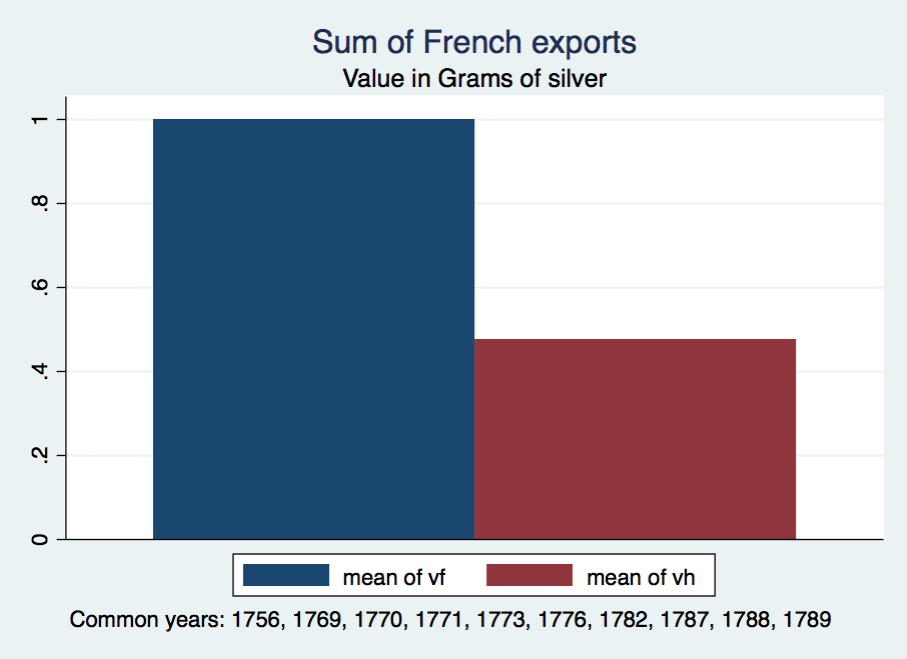
\includegraphics[scale=.28]{value_total_fr_hb_commonyears.png}
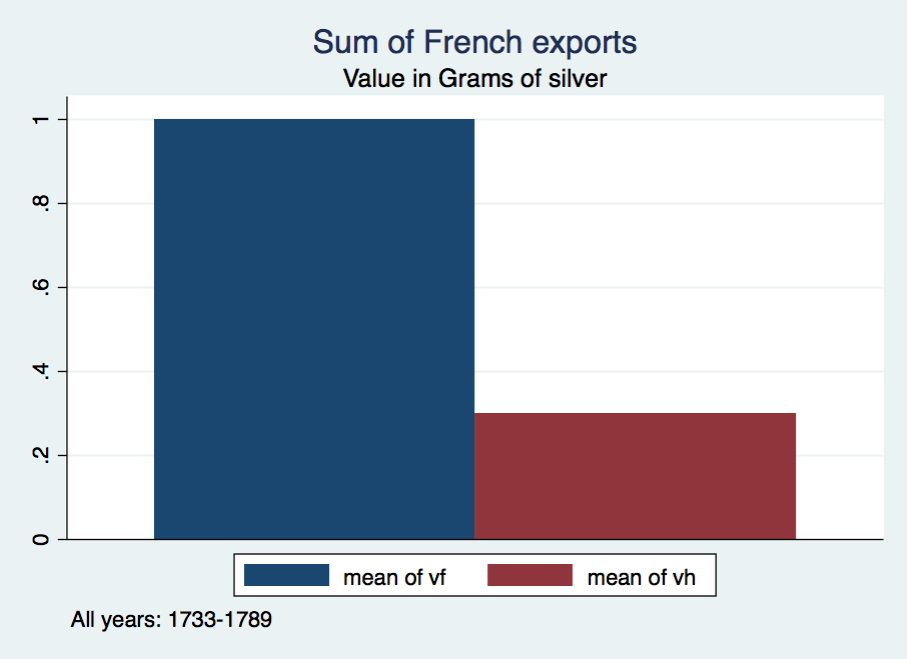
\includegraphics[scale=.28]{value_total_fr_hb.png}
Aggregate exports value in Hamburg source account for slightly less then 50\% of export value in the French source considering only common years and slightly around 30\% considering all years (1733-1789). The ratio of the two values however is far from stable; before 1740, the two sources report roughly the same value, Hamburg reports even more than France in 1735, which however might be due to the fact that the values I estimated for the period previous to 1753 for France are underestimating the real total value of exports. In the subsequent period there is a sharp decrease, and the ratio stabilizes around 5\%. Surprisingly, no major effect is evident in 1740 with the exclusion of Russia and in 1780, with the narrowing of the destination on the French dataset from “Nord” to “Hanseatic cities”. On the contrary, the ratio increases. This leads me to think either to a mistake in the data, or that the share meant for Russia was only a small part of the overall export towards North.

\begin{center}
\caption{Evolution of the ratio of datasets}
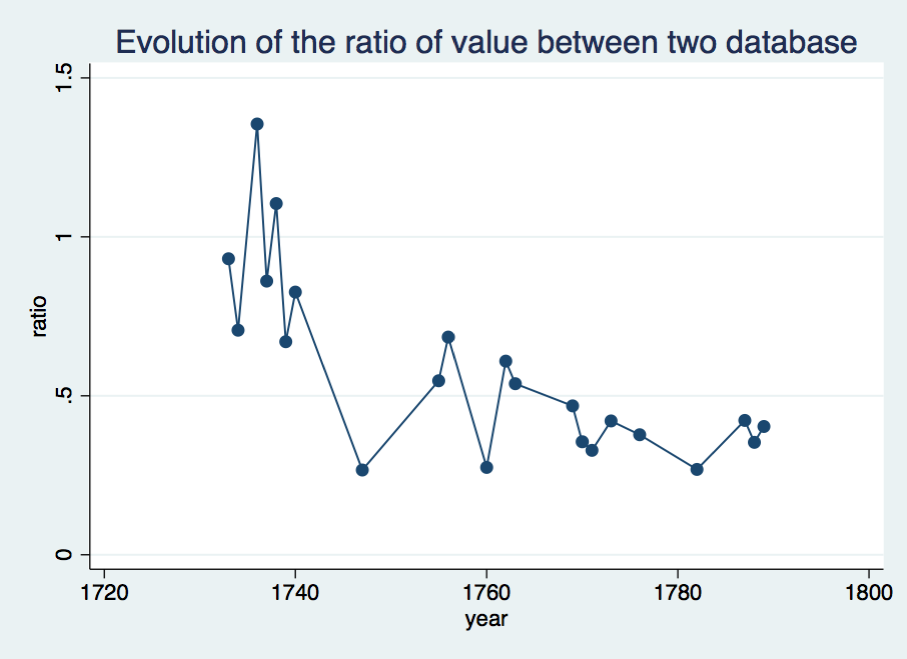
\includegraphics[scale=.3]{long_ratio.png}
\end{center}


\subsection{Comparison of total exports}
I will now turn to the evolution of aggregate exports per year.  For simplicity in comparison I have used value indexed at values in year 1787, which is the most complete for both sources. In this way I can observe better  the pattern of the two series, without considering the discrepancy in absolute value. 
From the graph below it is evident that the two sources move quite well together, with a correlation between the two series of 0.88. Also the data preceding 1740, which are an estimate, are in line with the Hamburg series. 
The overall trend of both series looks like an increasing one even though the growth is interrupted during war period. The Polish succession war between 1733 and 1738, did not seem to impact trade as much as colonial wars, whose effect on the other hand is very evident in the sharp decrease in 1761 and 1781. In this respect, I will go more into details in subsequent sections.

\begin{center}
\caption{Comparison of longitudinal evolution of aggregate exports}
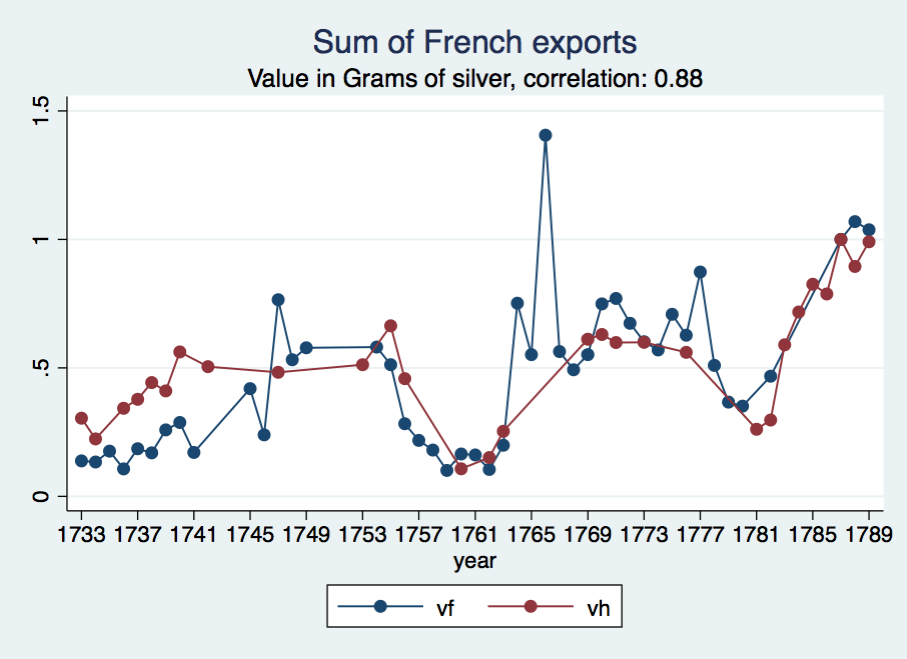
\includegraphics[scale=.3]{long_evolution.png}\\~\\
\end{center}

\subsection{Comparison at sector level}
\subsubsection{Comparison of aggregate export by sector}
The comparison at sector level brings contrasting results. At aggregate level the two sources are very close, both for the whole period and common years. It is evident that the major sector is exotic foodstuff, followed by beverages and tobacco and then by raw material, which however represents a significantly smaller share. Colonial imports are actually representing the biggest source of trade, which explains why then colonial wars were the cause of trade collapse. \\~\\
\caption{Comparison of total exports}
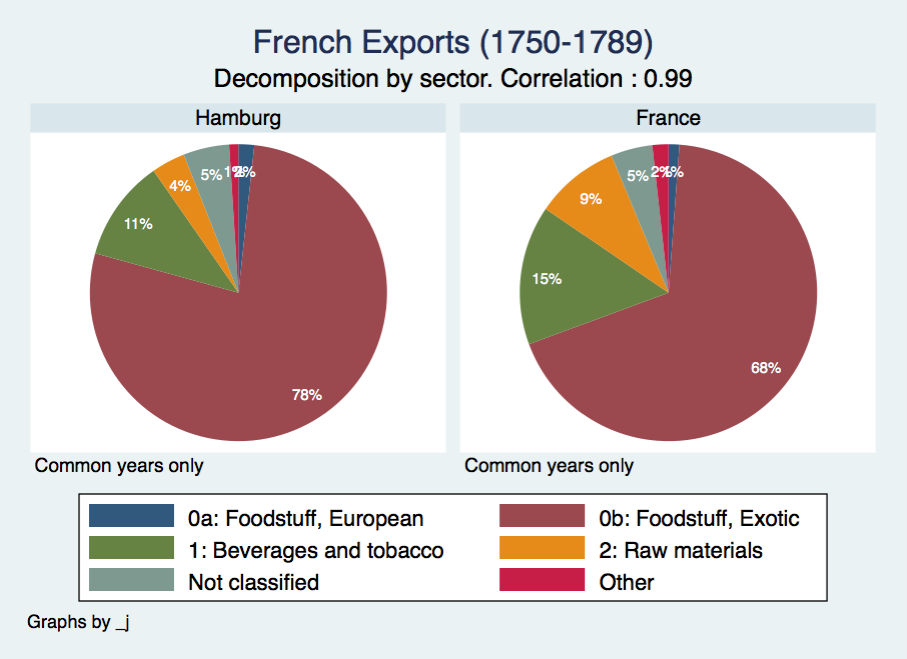
\includegraphics[scale=.28]{commonyears_sector.png}
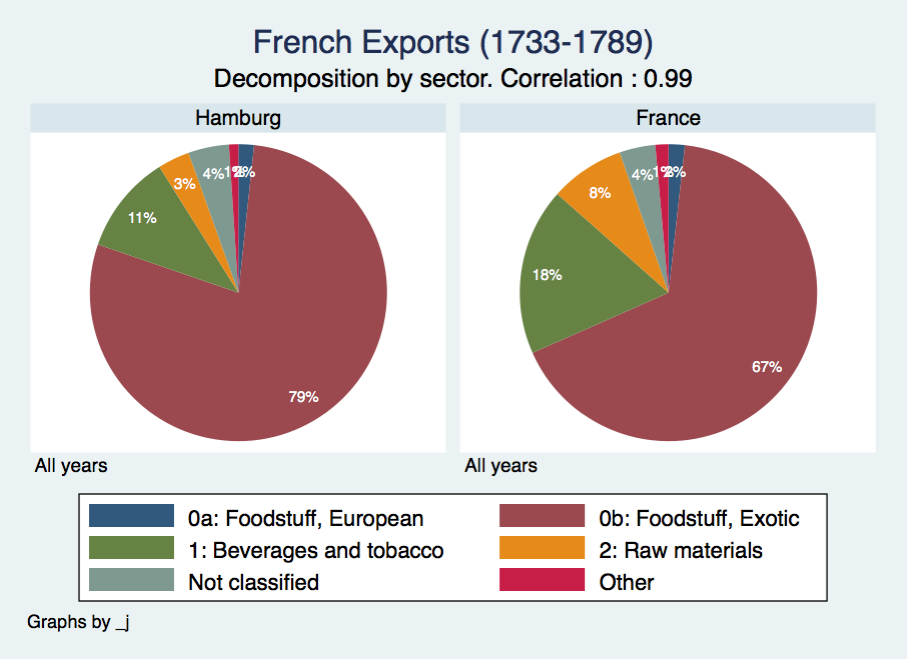
\includegraphics[scale=.28]{allyears_sector.png}

\subsubsection{Comparison of the evolution of major sectors overtime}
As mentioned above the three major sectors are Exotic foodstuffs, beverages and tobacco and raw material, with a higher importance given to the first two. The tables below plot the longitudinal evolution of these sectors according to the two different sources. Results are not as satisfactory as in the total exports longitudinal evolution above and it might be the case the estimation on the values of product pre-1750 was not too accurate because of lack of data. In all the three cases displayed below, I plotted both the share of the sector on the total and the absolute value (indexed at the 1787 value). 
\caption{Evolution of Exotic foodstuff}
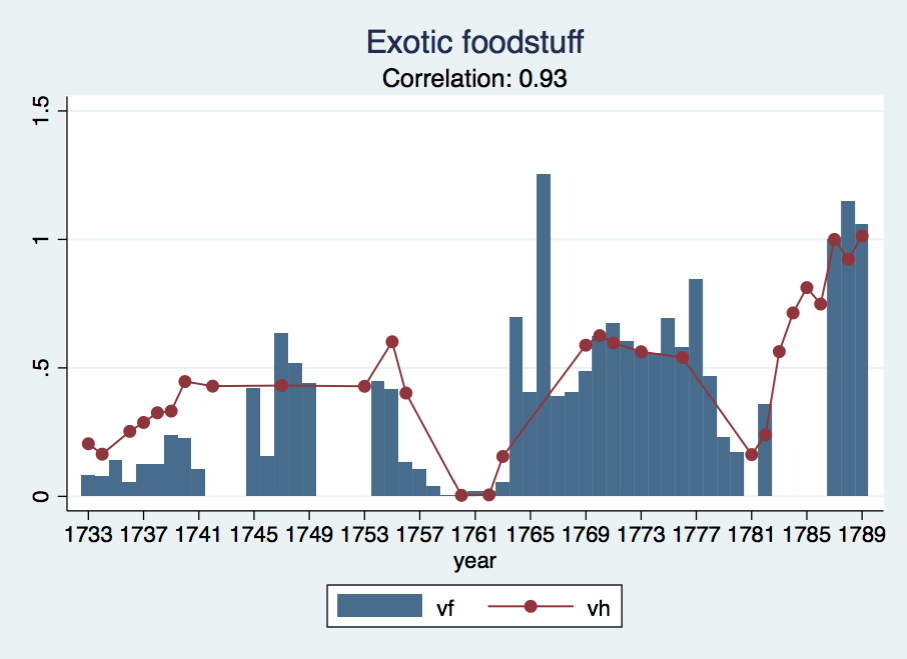
\includegraphics[scale=.28]{exotic_food_long.png}
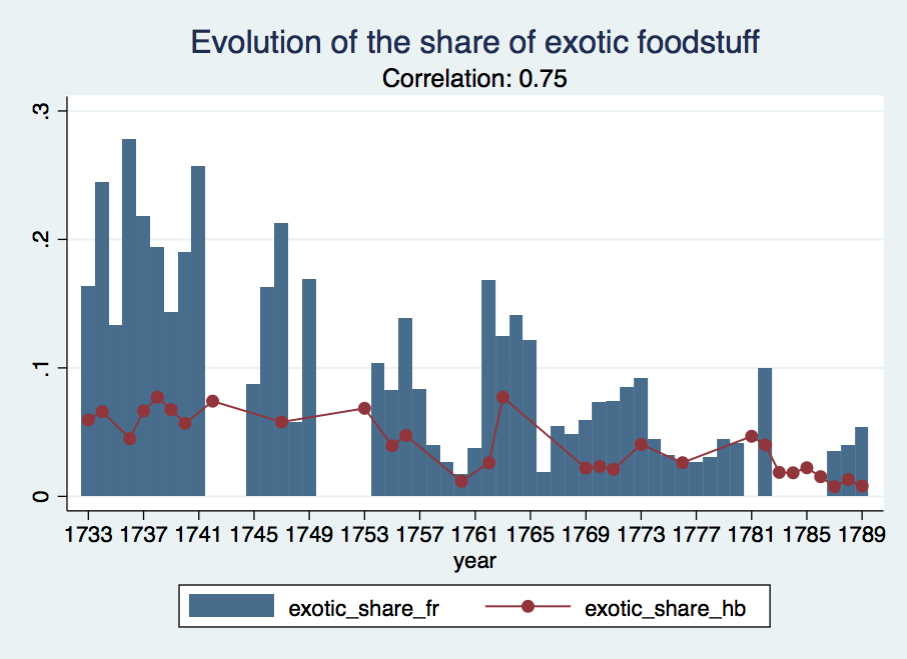
\includegraphics[scale=.28]{exotic_food_share.png}\\
\caption{Evolution of Beverages and Tobacco}
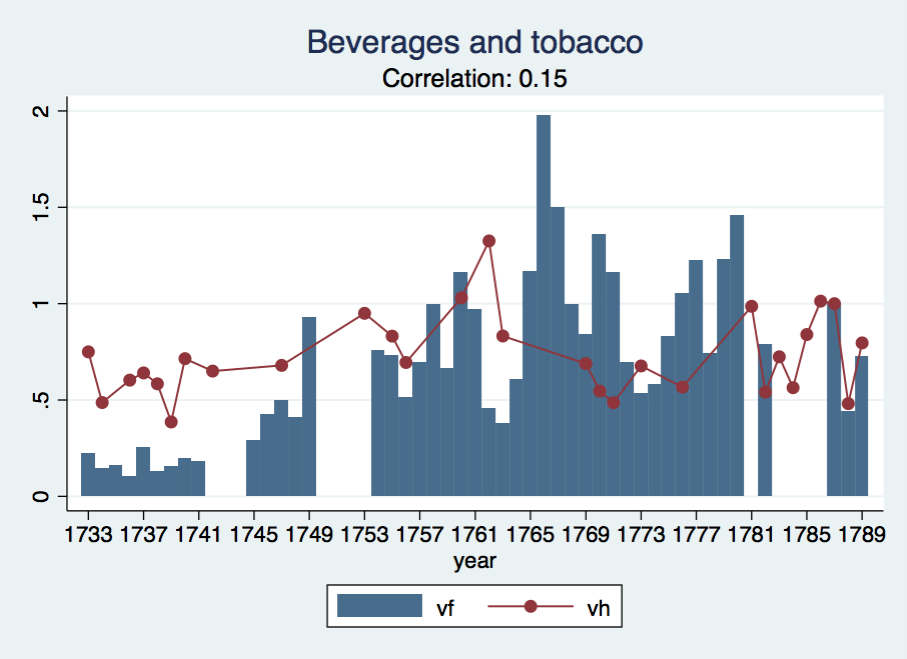
\includegraphics[scale=.28]{bev_tobacco_long.png}
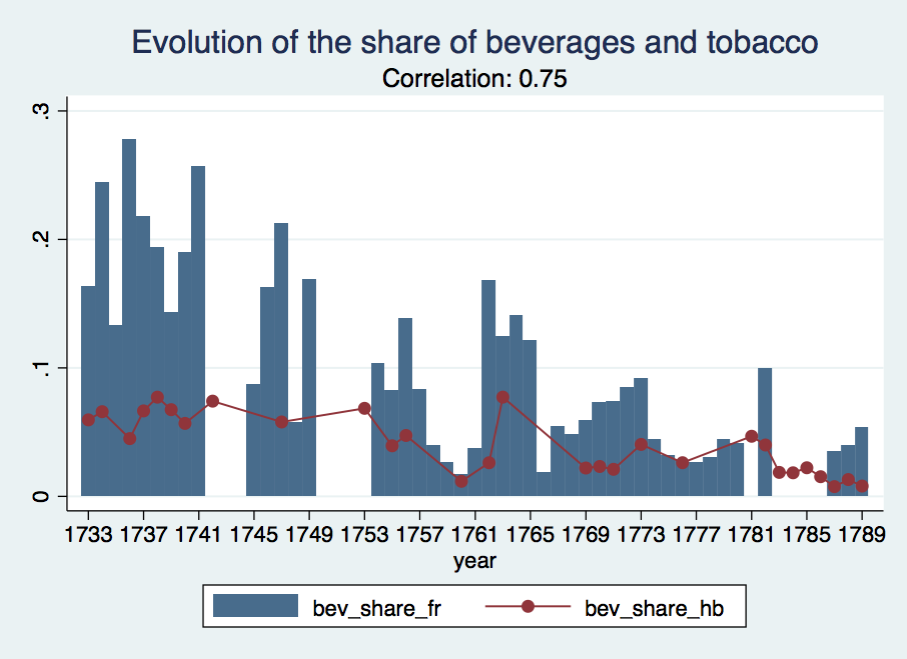
\includegraphics[scale=.28]{bev_tobacco_share.png}\\
\newpage
\caption{Evolution of Raw material}
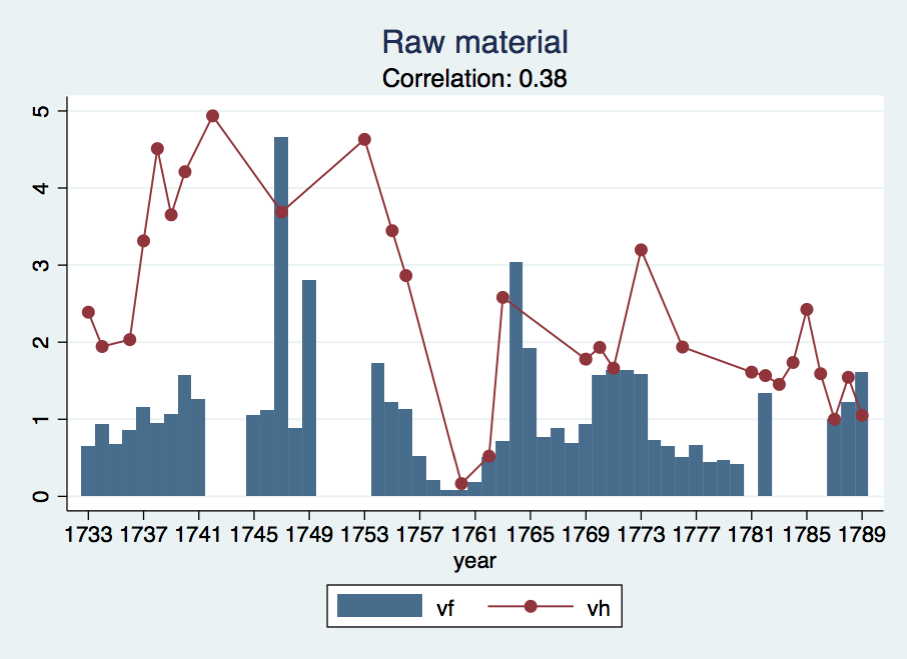
\includegraphics[scale=.28]{raw_mat_long.png}
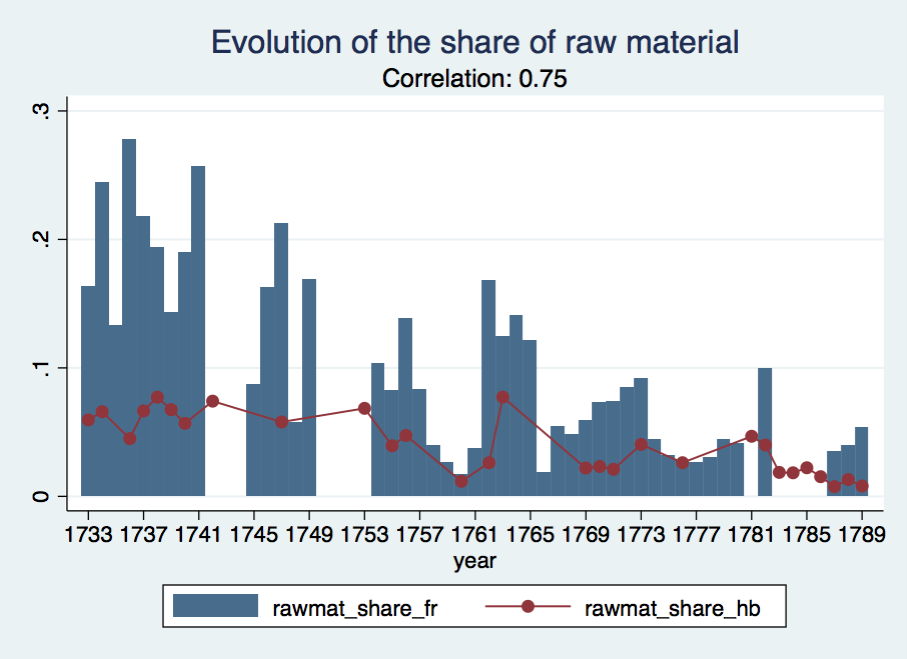
\includegraphics[scale=.28]{rawmat_share.png}

\subsection{Comparison at product}
\subsubsection{Comparison of aggregate export by product}
As for the case of sectors, products do not always give the results we would expect. At aggregate level both on all years and common years the two databases are quite close:\\~\\
\caption{Evolution of coffee}
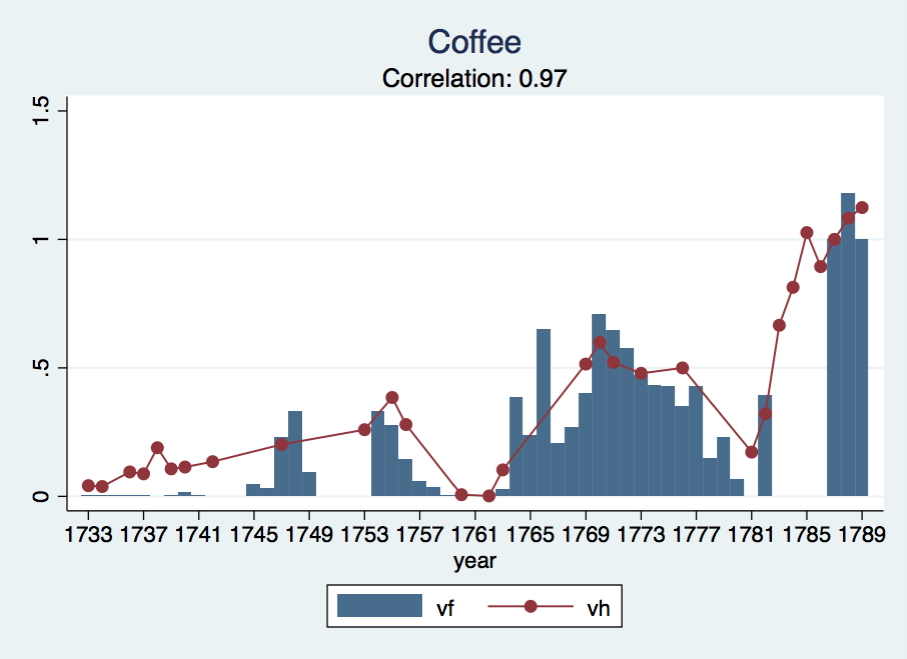
\includegraphics[scale=.28]{coffee_long.png}
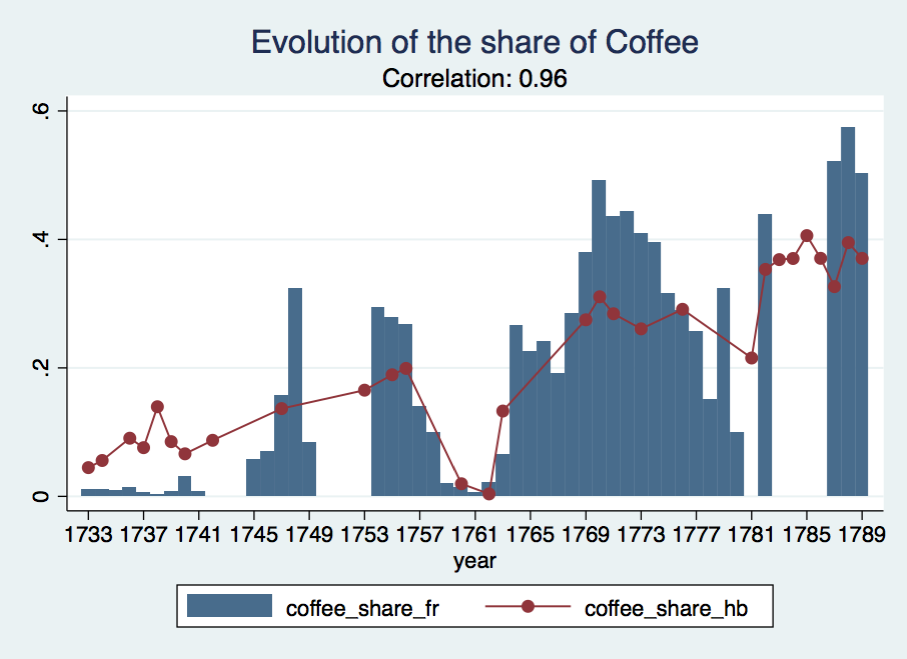
\includegraphics[scale=.28]{coffee_share_long.png}\\
\newpage
\caption{Evolution of Sugar}
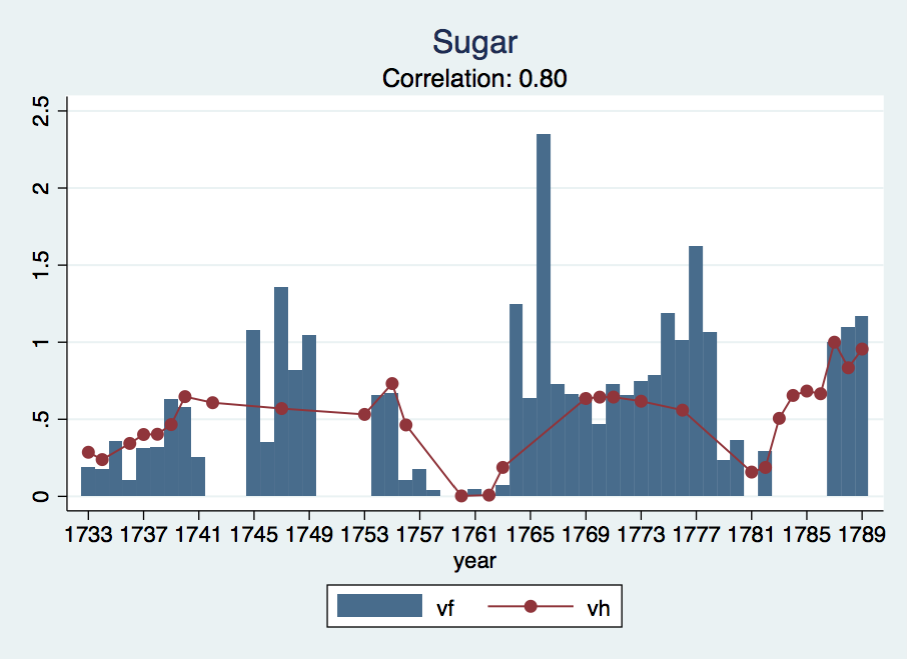
\includegraphics[scale=.28]{sugar_long.png}
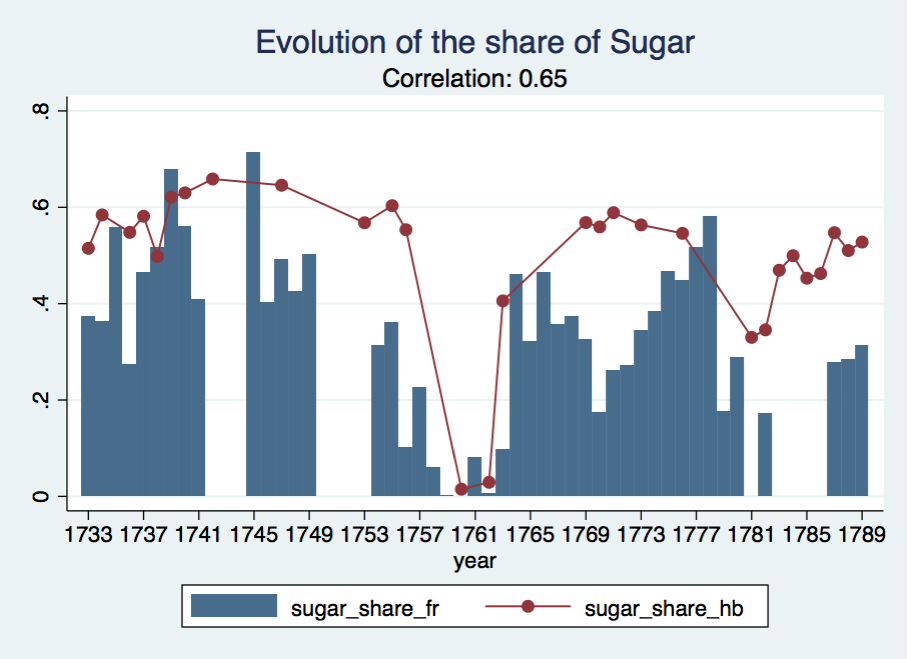
\includegraphics[scale=.28]{sugar_share_long.png}\\
\caption{Evolution of Indigo}
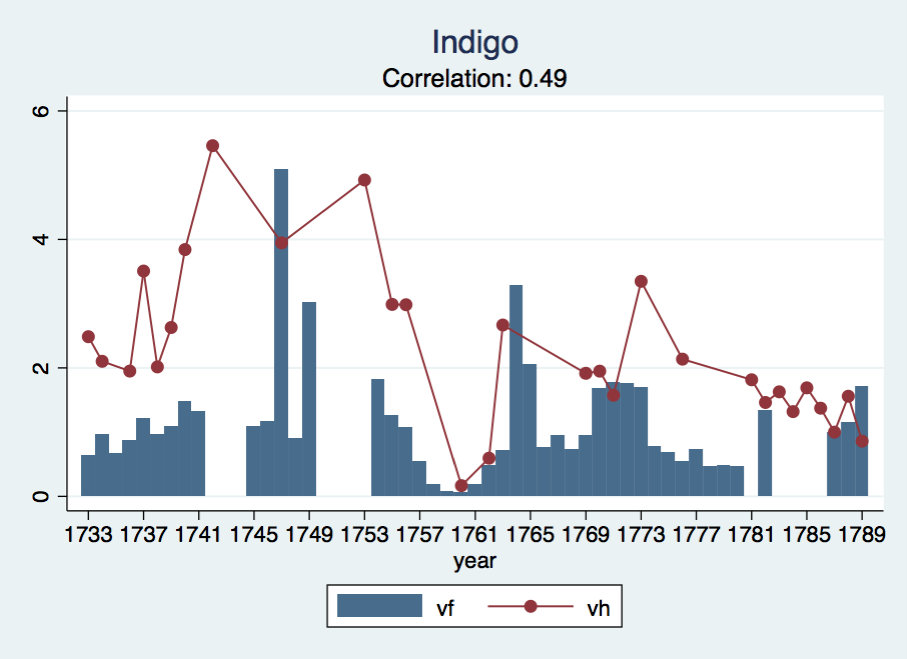
\includegraphics[scale=.28]{indigo_long.png}
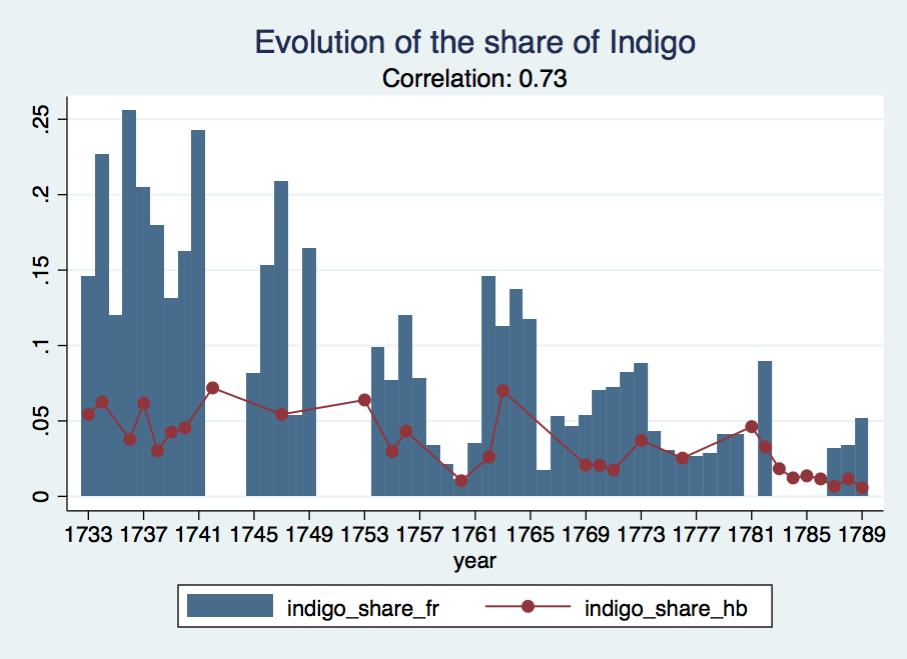
\includegraphics[scale=.28]{indigo_share_long.png}\\
\caption{Evolution of Eau de vie}
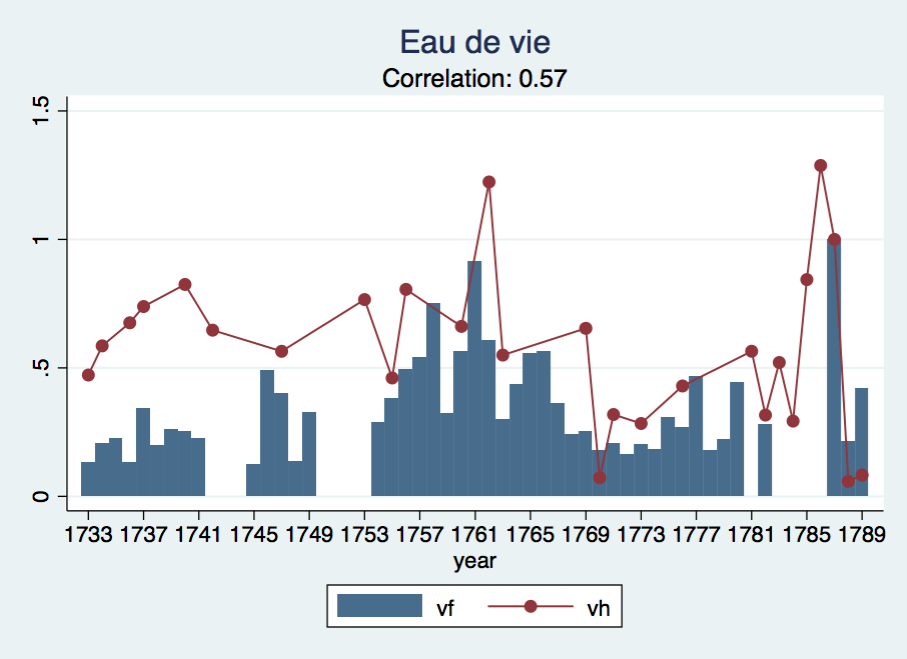
\includegraphics[scale=.28]{eaudevie_long.png}
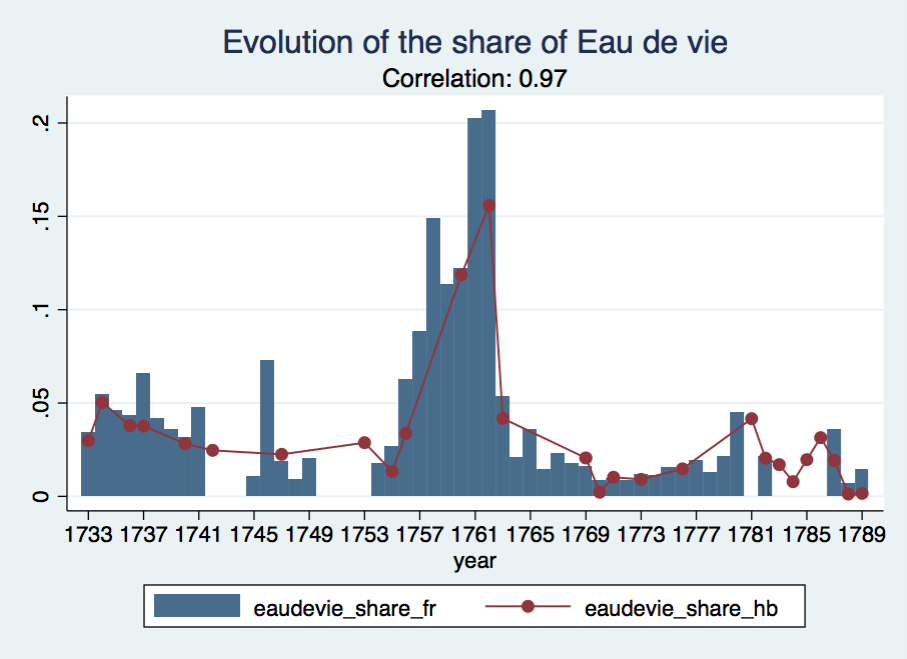
\includegraphics[scale=.28]{eaudevie_share_long.png}\\
\caption{Evolution of wine}
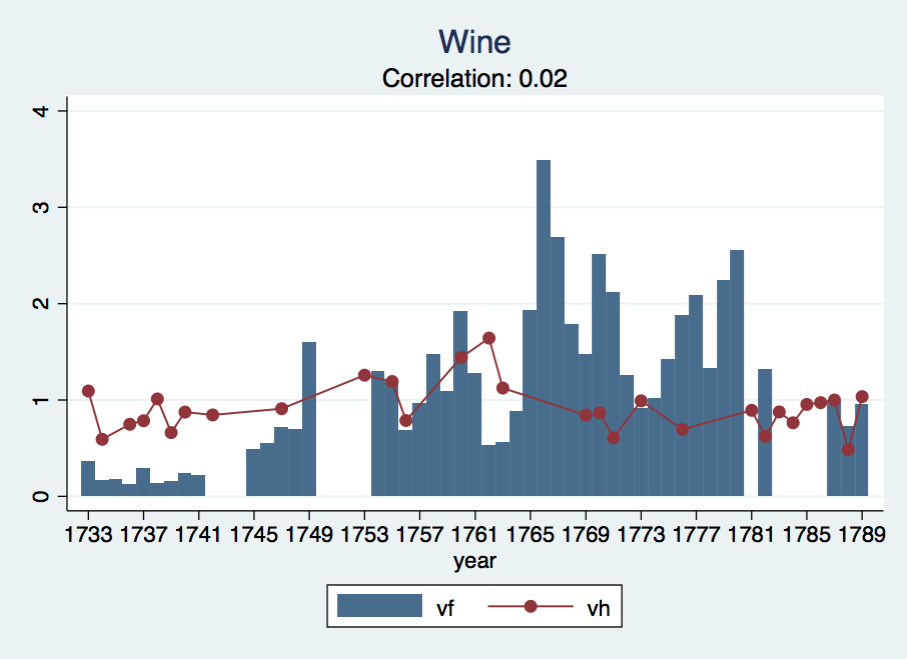
\includegraphics[scale=.28]{wine_long.png}
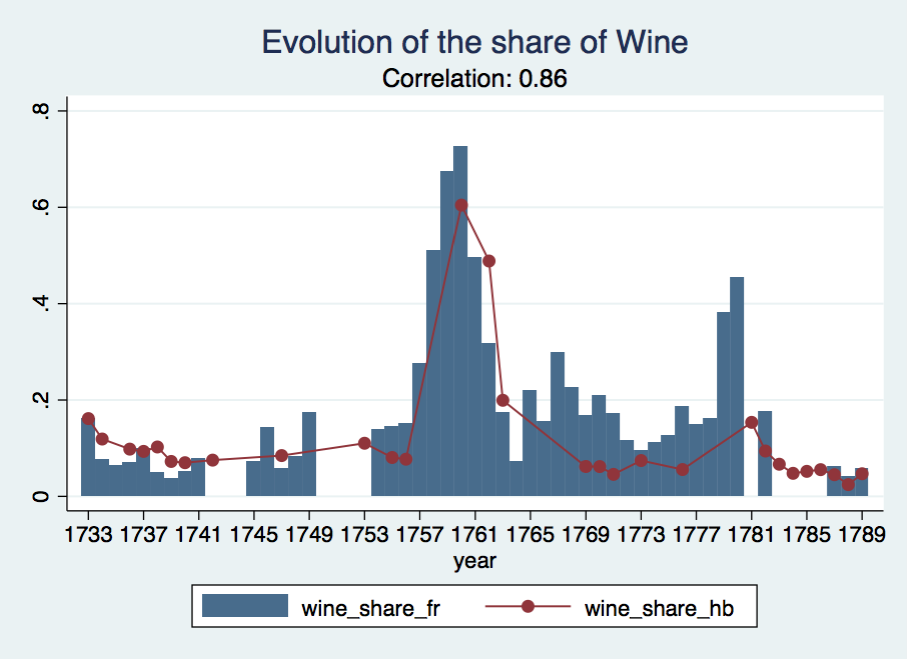
\includegraphics[scale=.28]{wine_share_long.png}
The evolution of sugar is not too precise comparing the two sources but overall the pattern is quite similar. The fact that strikes the attention is that sugar went to a nearly zero level during Seven Years War (both in share and absolute value) but experienced a less sharp decrease during the American revolutionary war. This pattern is also common to coffee and to a lesser extent to Indigo. On the contrary, in the case of wine and eau de vie, we observe an increase in export, even in absolute value, corresponding to the beginning of the Seven Years War, and then again a decline towards the end of the war. The increase in absolute value lasts till 1761 and then it also collapses together with coffee and sugar, however it remains the major source of export for the war period, especially in terms of share of overall exports. A similar pattern can be noticed during American revolutionary war but on a smaller scale. 

\subsection{Testing Benford’s law}
As a last step in my validation of the data, I have tested Benford’s law or the first-digit law on both datasets. Benford’s law is a law providing the frequency distribution of the first digit in most real life datasets. According to Benford the leading digit $d$, with $d \in \{1,...,9\}$ should follow the probability distribution: 
\begin{center}
$P(d)=\log_b(1+\frac{1}{d})$
\end{center}
where $P(d)$ is proportional to the distance between $d$ and $d+1$ on a logarithmic scale, which is the case when the logarithm of the numbers and not the numbers themselves are uniformly and randomly distributed. I run the following Pearsons’s chi square test:
\begin{center}
$$\chi^2=N\sum_{d=1}^{9}\frac{(p(d)-d(b))^2}{d(b)}$$
\end{center}
where N is the frequency and $p(d)$ and $d(b)$ are the proportions of Benford’s law and my data respectively. For both dataset I cannot reject the null hypothesis that the leading digit is actually distributed according to Benford’s law.
\caption{Benford'law}
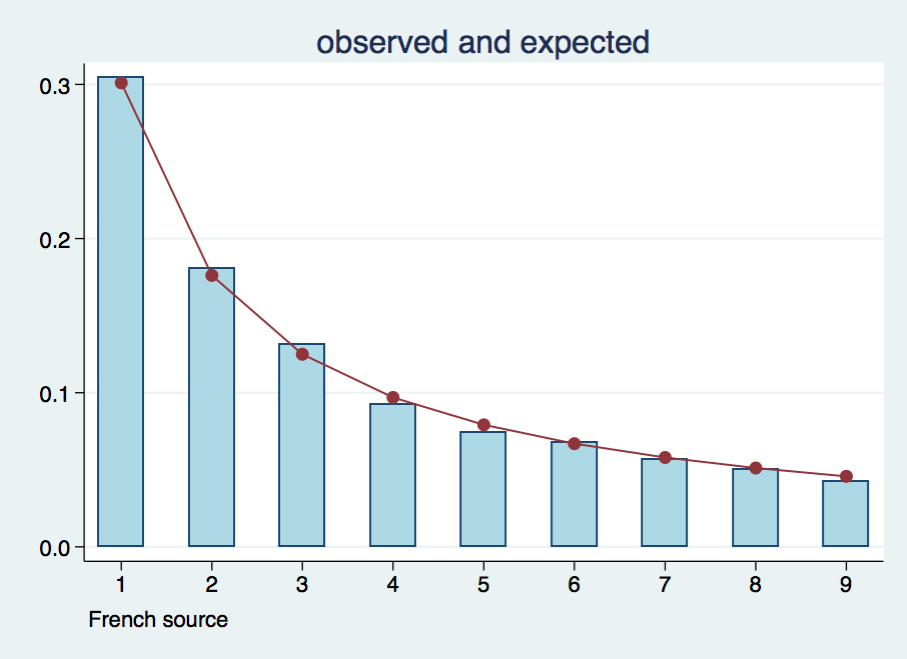
\includegraphics[scale=.28]{benford_fr.png}
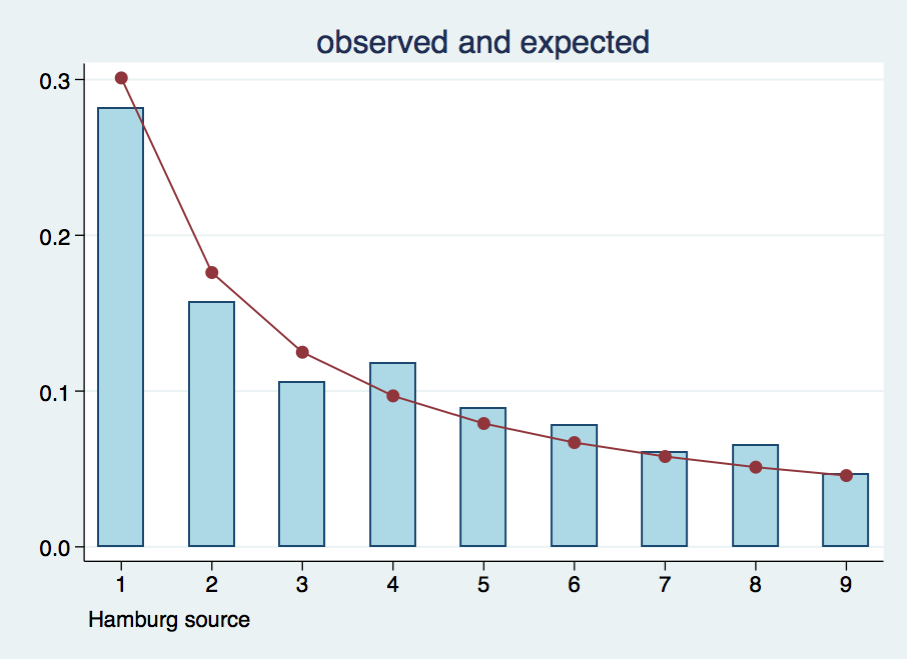
\includegraphics[scale=.28]{benford_hb.png}

\section{Analysis of trend of exports and effect of war}
From the series shown above, it is evident that trade towards Hamburg kept increasing according to both sources. However, if we look at the entire period, available only in the French dataset, the trend looks more quadratic and decreases starting 1800. 
\begin{center}
\caption{Rate of growth}
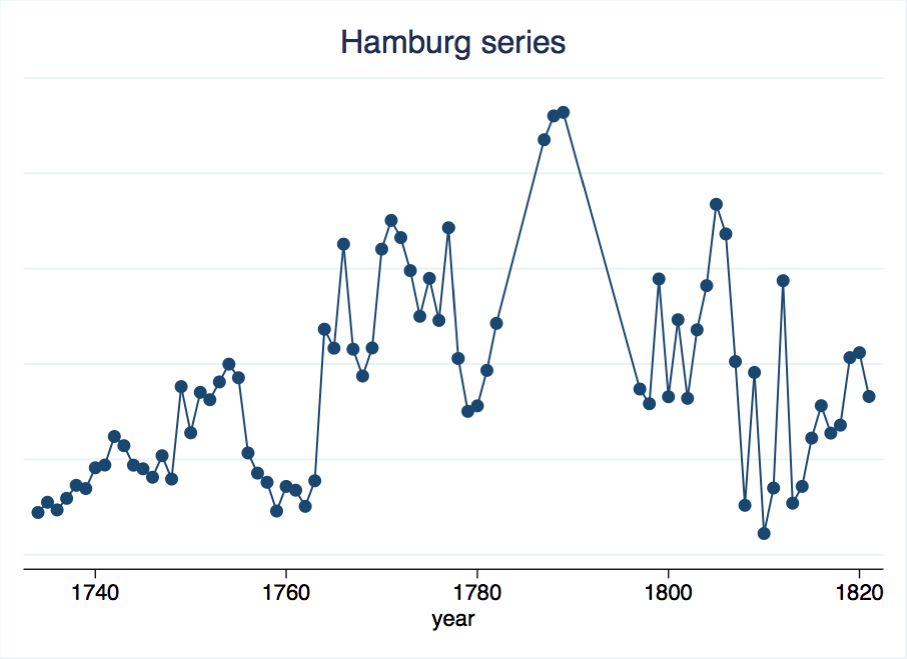
\includegraphics[scale=.35]{growth_rate.png}
\end{center}
We now want to look in details at the impact of historical events on exports, more precisely the effect of wars. There were seven major conflicts that hit Europe between 1733 and 1820; The War of the Polish succession (1733-1738), The War of the Austrian Succession (1740-1748), The Seven Years war (1756-1763), The American Revolutionary War (1775-1783), The French Revolutionary War (1792-1803) and The Napoleonic War (1803-1814). The Polish succession war and the first part of the Austrian succession war were mainly fought in Europe whereas the second half of Austrian succession war (1744-1748) and the other four wars were so called colonial wars, which defined the start of a new period in eighteenth century (Carrière 1973). In all the cases, France was a belligerent country whereas Hamburg was a neutral city. So we are interested in the impact of conflicts on neutral countries in particular. Normally, neutral countries in wartime were allowed to continue their trade with all other countries, disregarding the presence of a conflict.  This rule, however, had induced belligerent countries to exploit neutral ships for trading their own merchandises (Carrière 1973). For this reason, in the beginning of Seven Years War the British decided to put an end to this practice and produced a law stating that the nationality of the ship was not relevant, but what made it or not an enemy ship was the nationality of the cargo. This fact had a considerable impact on the trade of France, who had started to use Dutch ships to transport colonial goods, but also for all other neutral countries, who were clearly showing their discontent against this new British law. Those countries, nonetheless, were not united in their protest and could not really concretize their disappointment as a unique voice. Only in 1780, a League of Armed Neutrality was created. This experiment however did not have much success in its purposes and was finally put to an end in 1783 with the treaty of Paris, when Catherina of Russia renamed it the \textit{Armed Nullity} (Griffiths, 1971). 
All this brings me to think that we should expect a strong effect of conflicts on neutral countries. 
In what follows we will give a brief description of the four conflicts and then we will proceed in the analysis of their effects on exports. 

\subsection{Historical summary}
\subsubsection{War of Polish Succession}
The war of Polish succession took place between 1733 and 1738. It started with the death of the king of Poland August II who died heirless and soon become a conflict at European level. France, Prussia and Spain were trying to limit the desire of expansion of the Habsburg monarchy, which was aiming at extend its power over Poland. The lack of support by England however, concluded the war in 1738, with the recognition of August III as king of Poland. The belligerent countries were France, Spain and Italy on the one side and the Habsburg Monarchy on the other. 

\subsubsection{War of Austrian Succession}
The war of Austrian succession was a European conflict that burst in 1740 over the eligibility to succession to the crown of Maria Theresa of Austria, as the heir of the Habsburg Monarchy after the death of her father. It started out as a European conflict but after 1744 it involved also the colonies. Belligerent countries were France, Spain, Prussia and Italy on one side and England, Habsburg monarchy and the Dutch Republic on the other. 

\subsubsection{Seven Years Wars}
The Seven year war was a major conflict, which took place between 1756 and 1763. It is consider the first real world conflict and European powers were fighting over possession of colonies. Belligerents countries were: England, Prussia and Portugal on one side and France, Spain, Habsburg monarchy, and Dutch Republic on the other. 

\subsubsection{American Revolutionary War}
The American Revolutionary War took place between 1778 and 1782. In this case the field of battle was not Europe anymore, but directly the Colonies. British North American colonies were rebelling against Britain control over their trade and were fighting for independence. Belligerent countries were England on the one side and France, Spain and British Colonies on the other (later United States). During this war the First League of Armed Neutrality was signed between Russia, Sweden and Denmark. Spain accepted this agreement however Britain demurred. When Dutch Republic was about to join this league, Britain found out before the treaty was signed and captured a Dutch ships, thus forcing the Dutch to enter war against them. Starting 1781 therefore, the Dutch Republic also became a belligerent country, allied to France. 

\subsubsection{French Revolutionary Wars}
The French Revolutionary Wars took place between 1792 and 1802. It was a conflict that had started as a consequence of French Revolution, in 1789, with the hope of spreading the revolutionary ideas around Europe. During this war, France and Spain were fighting against most of the rest of Europe, in particular Great Britain and the Hasburg Monarchy. France experienced an unexpected success in continental Europe, because of the raise in power of general Napoloen Bonaparte, however was on the other hand heavily defeated by the Royal Navy, thus loosing supremacy over the Mediterranean and also its colonies. This conflict was ended by the Treaty of Amiens in 1802, which started the only year of peace in Europe between 1792 and 1815.

\subsubsection{Napoleonic Wars}
The Napoleonic wars were a series of conflict between the French Empire of Napoleon I and  other countries, primarily led by the British, which took place in the years 1803 to 1815. Its consequences were the final defeat of Napoleon, and the First French Empire, and the rise of the British Empire as the world's premier power. On the other hand, this conflict contributed to spread all over Europe the nationalist and liberal ideas that were born during the French Revolution, despite the restoration of the monarchy in France and the decay of the Revolutionary principles. 

\subsection{Analysis of impact of conflict on Hamburg trade}
As a first step we have constructed a Poisson Pseudo Maximum Likelihood model with the value of exports flows towards Hamburg as a dependent variable and introducing a war dummy to capture the effect of wars. We did so first using only one dummy for all wars and then adding one dummy for each war. 
\begin{equation}
exports_t=\exp(\beta_0+\beta_1year+\beta_3war)
\end{equation}
\begin{multline}
exports_t=\exp(\beta_0+\beta_1year+\beta_3polish +\beta_4austrian1 +\beta_5 austrian2+ \\ + \beta_5seven + \beta_6american +\beta_7revolutionary+\beta_8napoleonic)
\end{multline}

where $exports$  is the value of exports per year and  $year$ is the time trend. We are using time trend rather than year fixed effects for the scarcity of data and because time fixed effects would be collinear with the war dummy otherwise.
In the war by war case, we have considered the Austrian Succession war as two different conflicts as to try to capture the difference between the colonial and non colonial phase.\\
From the first equation we find that wars overall had a negative impact on Hamburg trade, amounting to a fall of roughly 42\%. By breaking down the effect for each single war, we find a 78\% reduction in trade caused by the Polish war, a decrease of 56\% for the first part of the Austrian war and a decrease of 62\%, 69\%, 18\%, 11\% and 19\% for the second part of Austrian war, Seven year war, American Revolutionary war, French Revolutionary war and Napoleonic war respectively, with the latter three coefficients not significant. These results are quite striking and incoherent with the series observed above: the effect of the Polish war in fact are barely visible in the trend, even though our regression suggests they are the stronger ones, whereas the effects of the Seven Years War are not that disruptive, as one would expect. There are two possible explanations to this fact. The first is that the data for the period 1733 to 1750 are not very reliable, as they come from local sources which are incomplete, and they are only estimates of what the true value might have been, as explained in section 3. The second explanation is that in 1795, as a consequence of the Revolutionary Wars, France had lost Saint Domingue, which had proclaimed its independence from France and together with it, its main sources of export to the North: sugar and coffee. Therefore, what we observe after this date, is an incisive break in the trend of exports and, as a consequence, a decline in total trade towards Hamburg. To take into account this effect, we have run a Chow test, by adding to the previous regressions a break both in time trend and in fixed effects. This test shows that there is indeed a break in 1795 and after introducing it in the model, the effects of the different wars become more coherent with respect to the series plotted above. The effect of Polish war goes down to -8\% and the coefficient is insignificant whereas Seven Years War and revolutionary War result as the most disruptive ones, with a loss in trade of 62\% and 73\% respectively. 

\begin{table}[htbp]\centering
\def\sym#1{\ifmmode^{#1}\else\(^{#1}\)\fi}
\caption{Hamburg Aggregate\label{tab1}}
\begin{tabular}{l*{6}{D{.}{.}{-1}}}
\toprule
                    &\multicolumn{1}{c}{No breaks}&\multicolumn{1}{c}{One break}&\multicolumn{1}{c}{Two breaks}&\multicolumn{1}{c}{No breaks}&\multicolumn{1}{c}{One break}&\multicolumn{1}{c}{Two breaks}\\
\midrule
Value               &                     &                     &                     &                     &                     &                     \\
All                 &      -0.545\sym{***}&      -0.613\sym{***}&      -0.618\sym{***}&                     &                     &                     \\
Polish              &                     &                     &                     &      -0.197         &      -0.625\sym{***}&      -0.330\sym{**} \\
Austrian1           &                     &                     &                     &      -0.818\sym{***}&      -0.207\sym{**} &      -0.876\sym{***}\\
Austrian2           &                     &                     &                     &      -0.979\sym{***}&      -0.491\sym{***}&      -1.046\sym{***}\\
Seven               &                     &                     &                     &      -0.207         &      -0.678         &      -0.678         \\
American            &                     &                     &                     &      -1.513\sym{***}&      0.0878         &      -0.102         \\
Revolutionary       &                     &                     &                     &      -0.120         &      -1.289\sym{*}  &      -1.289\sym{*}  \\
Napoleonic          &                     &                     &                     &      -1.173\sym{***}&      -1.053\sym{***}&      -1.267\sym{***}\\
\midrule
Observations        &          76         &          76         &          76         &          76         &          76         &          76         \\
Pseudo \(R^{2}\)    &       0.319         &       0.665         &       0.661         &       0.491         &       0.742         &       0.637         \\
\bottomrule
\multicolumn{7}{l}{\footnotesize \sym{*} \(p<0.05\), \sym{**} \(p<0.01\), \sym{***} \(p<0.001\)}\\
\end{tabular}
\end{table}


We also perform two different robustness checks for these results, using a log-linear model, (section 7) but they do not change significantly the coefficients of the regression. \\
On average we can say that wars were very disruptive for Hamburg trade, despite it being a neutral country, which does reflect what claimed by Glick and Taylor (2005), concerning effects of war even on neutral countries. One remark should be added however; wars in the first half of eighteenth century (until 1744, separation suggested by Carrière 1973), which were mostly non-colonial, had a smaller impact on Hamburg trade. This is a first interesting result, in the sense that, we see here that not all wars had the same effects; more specifically wars fought in Europe had smaller effects than wars fought also/only in the colonies. In our opinion an explanation has to be found in the fact that the major source of import for Hamburg was actually colonial products, the trade of which during colonial wars was interrupted. On the other, We believe that the trade of European products did not have such a strong interruption and that it might even be the case that given the impossibility to trade exotic products, the commerce of other goods might have developed more to compensate for losses. \\
To test this hypothesis, we have looked at exports flows disaggregated by products. We only consider the main two colonial products (sugar and coffee) and the main two European products (wine and eau de vie) plus one category (other), encompassing all the remaining 35 different goods. We run the following regression, interacting the product dummies with the war dummies, first with all wars in one dummy and then separately:
\begin{equation}
exports_i=\exp(\beta_0+\beta_1year+ 
\beta_2product_i + \beta_3product_iyear+\beta_4product_iwar)
\end{equation}
\begin{multline}
exports_i=\exp(\beta_0+beta_1year+\beta_2product_i + \beta_3product_iyear+\beta_4product_ipolish + \\ +\beta_4product_iaustrian1 + \beta_5product_iaustrian2 + \beta_6product_iseven +\beta_7product_iamerican+  \\ +\beta_8product_irevolutionary+\beta_8product_inapoleonic)
\end{multline}

where$year$ is again the time trend, $product_i$ is product fixed effect, $product_iyear$ is the product time trend and $product_iwar$ is the interaction of the product dummy with the war dummy, which is the coefficient of interest. As we mentioned before, it is reasonable to assume a break in 1795, and in this case, we can insert it for the products specifically concerned, i.e. sugar and coffee. Once more, both the time trend and the fixed effects Chow test are significant and they yield more sensible estimates. Table 19 shows the results of the regression with no break, with one break only for coffee and with breaks for both sugar and coffee. \\
The impact of conflicts in general on colonial products was significantly greater, -76\% for coffee and -68\% on sugar, whereas the impact on wine is definitely smaller and insignificant and exports of eau de vie is even positive and very big in size (+7\% and +300\% respectively).
Given these first results, we can indeed say that the disruption in trade was led by the collapse of colonial products, but some European products, on the other hand, were even benefiting from conflicts. It is in fact evident from the graph shown below that to the collapse of sugar and coffee 1795 there is a corresponding peak in the export of wine and eau de vie.\\~\\
\caption{\textbf{Inverse trends of European and Colonial products}}
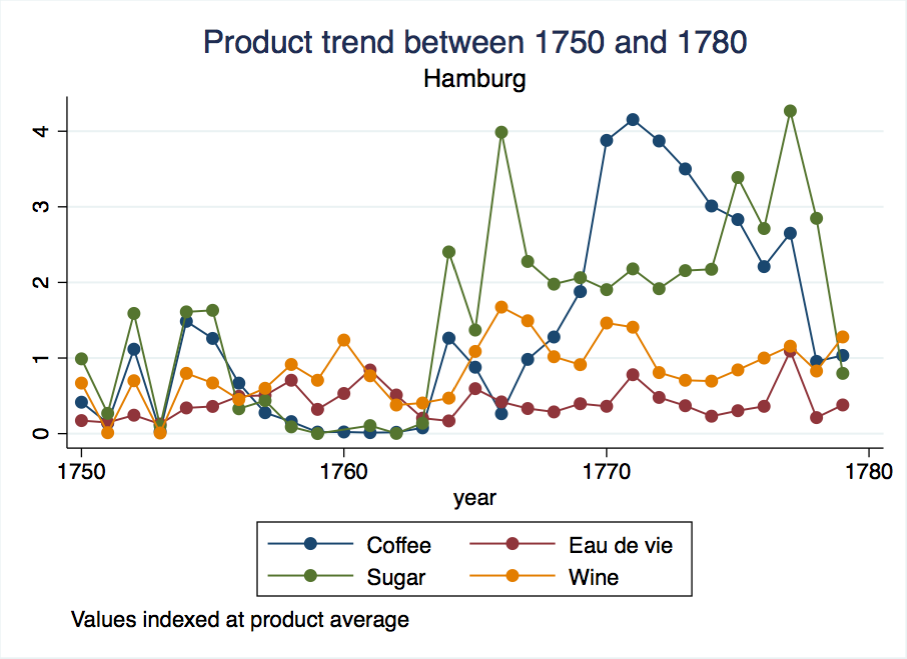
\includegraphics[scale=.35]{hamburg_product_1780.png}
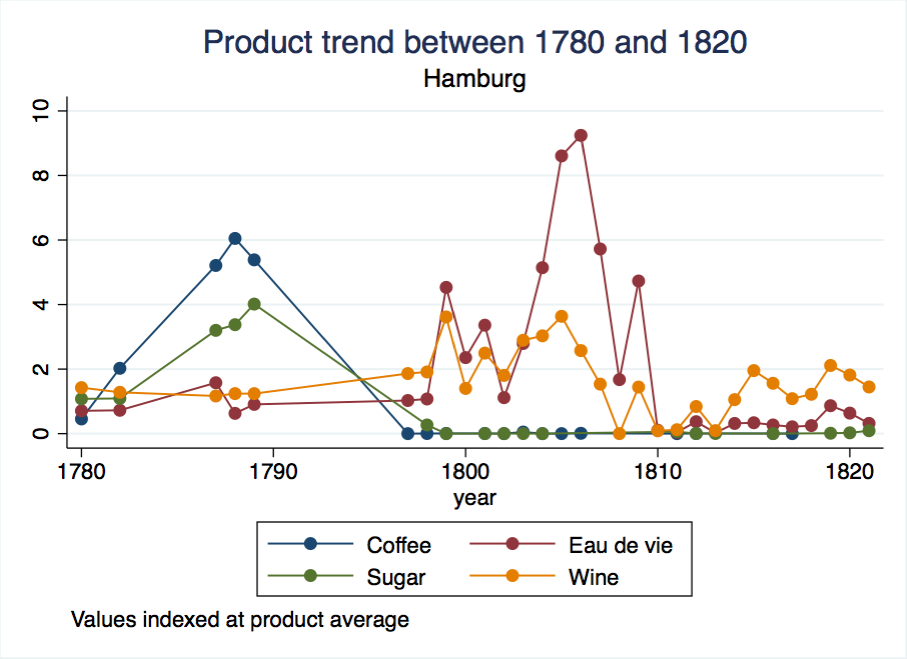
\includegraphics[scale=.35]{hamburg_product_1820.png}\\~\\
Turning to the war by war case, results are less well-defined. The impact of each war is indeed negative but not necessarily sugar and coffee are more impacted than wine and eau de vie and we are no more able to disentangle the effects of colonial and non-colonial conflicts that precisely. Adding the break for coffee and sugar does not change the picture too much, and in this instance only the Chow test for coffee is significant. Nonetheless, it is interesting to notice that, when considering only the break for coffee, on average, wine and eau de vie are more strongly impacted during Polish and Austrian war, whereas sugar and coffee show a bigger decrease during the Seven Years war and the subsequent wars. We can therefore state, that also in this case, even in a less clearcut way, we can observe the difference in impact depending on the kind of wars. As for the aggregate case, the size of the coefficient for the wars preceding 1750, might be biased by the inaccuracy of our estimation and the incompleteness of data, which is not corrected for by adding a break, in this case. 
An interesting point to remark is that, by looking at the wine time series in section 4, we also notice an interesting pattern during Seven Years War, increasing initially and then decreasing during the second half of the conflict.  We will not analyse this issue more in detail here but it could be the object of further research. 
\begin{table}[htbp]\centering
\def\sym#1{\ifmmode^{#1}\else\(^{#1}\)\fi}
\caption{Hamburg: All wars on each product\label{tab1}}
\begin{tabular}{l*{3}{D{.}{.}{-1}}}
\toprule
                    &\multicolumn{1}{c}{No breaks}&\multicolumn{1}{c}{One break}&\multicolumn{1}{c}{Two breaks}\\
\midrule
Value               &                     &                     &                     \\
Coffee              &      -2.436\sym{***}&      -1.403\sym{***}&      -1.444\sym{***}\\
Eau de vie          &       1.387\sym{***}&       1.387\sym{***}&       1.387\sym{***}\\
Sugar               &      -1.874\sym{***}&      -1.874\sym{***}&      -1.136\sym{***}\\
Wine                &      0.0711         &      0.0711         &      0.0711         \\
Product FE          &         Yes         &         Yes         &         Yes         \\
Product time trend  &         Yes         &         Yes         &         Yes         \\
Break Coffee        &          No         &         Yes         &         Yes         \\
Break Sugar         &          No         &          No         &         Yes         \\
\midrule
Observations        &         347         &         347         &         347         \\
Pseudo \(R^{2}\)    &       0.460         &       0.559         &       0.645         \\
\bottomrule
\multicolumn{4}{l}{\footnotesize \sym{*} \(p<0.05\), \sym{**} \(p<0.01\), \sym{***} \(p<0.001\)}\\
\end{tabular}
\end{table}

\begin{table}[htbp]\centering
\def\sym#1{\ifmmode^{#1}\else\(^{#1}\)\fi}
\caption{Hamburg: Each wars on each product\label{tab1}}
\begin{tabular}{l*{3}{D{.}{.}{-1}}}
\hline\hline
                    &\multicolumn{1}{c}{No breaks}&\multicolumn{1}{c}{One break}&\multicolumn{1}{c}{Two breaks}\\
\hline
Value               &                     &                     &                     \\
0                   &           0         &           0         &           0         \\
Polish Coffee       &      -8.087\sym{***}&      -2.052         &      -6.442\sym{***}\\
Polish Eau de vie   &      -5.869\sym{***}&      -5.869\sym{***}&      -5.869\sym{***}\\
Polish Sugar        &      -4.088\sym{***}&      -4.088\sym{***}&      -2.545\sym{***}\\
Polish Wine         &      -10.70\sym{***}&      -10.70\sym{***}&      -10.70\sym{***}\\
Austrian1 Coffee    &      -8.217\sym{***}&      -2.109         &      -6.749\sym{***}\\
Austrian1 Eau de vie&      -5.740\sym{***}&      -5.740\sym{***}&      -5.740\sym{***}\\
Austrian1 Sugar     &      -3.806\sym{***}&      -3.806\sym{***}&      -2.504\sym{***}\\
Austrian1 Wine      &      -11.25\sym{***}&      -11.25\sym{***}&      -11.25\sym{***}\\
Austrian2 Coffee    &      -5.104\sym{***}&      -3.777\sym{***}&      -3.920\sym{***}\\
Austrian2 Eau de vie&      -4.510\sym{***}&      -4.510\sym{***}&      -4.510\sym{***}\\
Austrian2 Sugar     &      -3.165\sym{***}&      -3.165\sym{***}&      -2.135\sym{***}\\
Austrian2 Wine      &      -10.03\sym{***}&      -10.03\sym{***}&      -10.03\sym{***}\\
Seven Coffee        &      -2.345\sym{***}&      -1.883\sym{**} &      -1.855\sym{**} \\
Seven Eau de vie    &       0.222         &       0.222         &       0.222         \\
Seven Sugar         &      -2.372\sym{***}&      -2.372\sym{***}&      -2.005\sym{***}\\
Seven Wine          &    -0.00508         &    -0.00508         &    -0.00508         \\
American Coffee     &      -0.636         &      -1.170\sym{***}&      -1.171\sym{***}\\
American Eau de vie &       0.357         &       0.357         &       0.357         \\
American Sugar      &     -0.0691         &     -0.0691         &      -0.695\sym{*}  \\
American Wine       &       0.361\sym{**} &       0.361\sym{**} &       0.361\sym{**} \\
Revolutionary Coffee&      -6.611\sym{***}&       0.721         &      -4.914         \\
Revolutionary Eau de vie&       1.812\sym{***}&       1.812\sym{***}&       1.812\sym{***}\\
Revolutionary Sugar &      -3.157\sym{***}&      -3.157\sym{***}&      -0.556         \\
Revolutionary Wine  &       0.608\sym{***}&       0.608\sym{***}&       0.608\sym{***}\\
Napoleonic Coffee   &      -5.690\sym{***}&       1.797         &      -1.912         \\
Napoleonic Eau de vie&       2.160\sym{***}&       2.160\sym{***}&       2.160\sym{***}\\
Napoleonic Sugar    &      -4.739\sym{***}&      -4.739\sym{***}&      -1.583         \\
Napoleonic Wine     &      0.0339         &      0.0339         &      0.0339         \\
Cons                &      -12.69         &       17.36         &      -102.8\sym{***}\\
Product FE          &         Yes         &         Yes         &         Yes         \\
Product time trend  &         Yes         &         Yes         &         Yes         \\
Break Coffee        &          No         &         Yes         &         Yes         \\
Break Sugar         &          No         &          No         &         Yes         \\
\hline
Observations        &         347         &         347         &         347         \\
Pseudo \(R^{2}\)    &       0.589         &       0.659         &       0.716         \\
\hline\hline
\multicolumn{4}{l}{\footnotesize \sym{*} \(p<0.05\), \sym{**} \(p<0.01\), \sym{***} \(p<0.001\)}\\
\end{tabular}
\end{table}

In sum, from the estimations made so far, we can conclude that there was indeed an overall negative impact on Hamburg trade, but it was very product specific, with colonial products suffering more than others and European products benefiting from the conflict on the other hand.

\subsection{War lags}
****\textbf{Should I keep this part?}\\
The impact on European products was found strongly negative for European wars but not that significant in Colonial wars. These results are already in contrast with some of the literature (i. e. Glick and Taylor (2005) and Thierry, Martin and Mayer (2010)), which found generic negative impact on trade with no war-type or product-type differentiation. Only Blomberg and Hess (2004), have disentangled the impact of different kind of conflicts but they focused on external versus internal violence instead.\\
Another interesting issue which is extensively treated in the literature is the presence of war lags and slow trade recovery after conflicts. Glick and Taylor (2005) for instance, found major war lags for both neutral and adversary countries for a period up to ten years. We have tested their findings on our Hamburg series, adding to the above regressions dummies for lag from 1 to 5 years (tables are the appendix). We have opted for 5 years of lag because in this period trade was much more unstable and effects after five years might have been due to other unrelated issues. In addition, using 10 years lags would basically mean including another war period. For this same reason we are only looking at lags for the Austrian Succession war, Seven Years War and Napoleonic wars, and those three wars together (no data are available for the period immediately after American Revolutionary War). We have done so again on all wars together and on wars separately as before. Results are not very coherent across regressions. In the overall case, coefficients of lag dummies are negative, with the first and third year of lag being insignificant and smaller in size. Splitting the one war dummy into the five different wars, lags are alternating signs for the Austrian War and Seven Years War, starting with positive, but are constantly negative and significant for the Napoleonic War.
Turning to the breakdown by product, on the other hand, we notice that there is evidence of strong war lags for all products, interestingly enough, for eau de vie as well, which, during conflicts had experienced a strong increase. This might suggest that wars were boosting trade of certain products in the period of the conflict, which were then restoring their prewar trade level, after the conflict had stopped.\\
Overall we can say that we do not have a clear picture on the existence of war lags: there is evidence of some post-conflicts effect, however they are not always negative, significant or long lasting, as described in the literature. \\
\iffalse
This was also noted by Riley (1984), who analyses the case of the Seven Years War and claims that merchants were actually forecasting the wars (using price of lead) and stocking products to sell them at the end of the conflict, thus compensating for war losses. He also claims that this was not only happening after the wars but also before, so he saw an increase in exports before and after wars. I have tested his findings on my data by adding to the main regression a dummy for up to four years preceeding the conflict, as suggested by Riley (1984). In the general case (all wars in one dummy) coefficient are positive but very small, so Riley’s claim is not really reflected here. On the other hand, in the war-by-war case, coefficients for one year preceding conflict are positive and bigger in size, however it is not a constant effect throughout the four years. 
I have then run the same regressions by adding product fixed effects, as before, and introducing pre-war dummies interacted with products. Results do not differ much from the aggregate level; there is a constant positive effect one year before the war, which in this case it is more pronounced for European goods. In the war-by-war case finally, there is no big change with the results of the other regressions. \\
In short, I have found no evidence of war lags or loss in trade subsequent to the war, it looks more like trade increased after the war (all coefficient are positive) and even if it does not exactly overshoot, at least it recovered extremely fast its pre-war level and growth rate. 
\fi
In this section I have made four main points on the impact of war on Hamburg; 1) war is indeed a major source of trade disruption, 2) the impact however was mainly on colonial goods such as sugar and coffee, 3) there is no evidence of war lags but on the contrary trade increased following the conflict 4) It was not possible to disentangle precisely the effect of colonial versus non colonial wars. In next section I compare these findings with the case of overall exports of France towards all countries. \\



\subsection{Comparison with French total exports}
In this section we have compared the results obtained for Hamburg with the general case of all French trading partners in eighteenth century. We have run a difference in difference specification to see the difference in impact for neutral and adversary countries with respect to allies. As in the case of Hamburg, I have again incomplete data on products preceding 1750, so We have estimated the value for sugar coffee, wine and eau de vie through the same technique. \\
We started my analysis running the following equation for all wars together and separately:
\begin{equation}
exports_{i,t}=\exp(\beta_0+\beta_1year + \beta_2country_i+\beta_3country_iyear+\beta_4adversaries_i+\beta_5neutral_i)
\end{equation}

where $year$ is year time trend, $country$ is country fixed effects, $country_iyear$ is country time trends, $adversaries$ is a dummy variable that takes value 1 if a country is adversary to France during a conflict and $neutral$ is again a dummy indicating whether a country was neutral (rather than adversary or allied). Even in this case we did not have enough data to estimate country year fixed effects so we have used time trend.\\
From the first regression we can see that war had on average a negative impact on trade of neutral countries of around 31\%. As for the case of Hamburg, we have run a Chow test for the year 1795, first for all countries and then for those countries importing mainly colonial goods. The test is significant for all countries and the result do not change much from one specification to the other. 
By looking at each single war separately, we notice that the difference in impact between colonial and non colonial wars is not really evident anymore, even after inserting the 1795 break. The first three wars, Polish Austrian 1 and 2, seem to have the biggest impact, whereas the subsequent colonial wars have a minor effect. As mentioned before, we suspect that this is due to imprecisions in the data. \\
Overall the impact for all wars is indeed negative and this finding is line with Hamburg case, discussed previously. However, loss estimated for neutral countries are less striking than the ones found for Hamburg and in particular, they are distributed differently  in the war by war case.
For this reason I have looked again into the breakdown by the major products and analysed the impact of wars on different goods. I am arguing that in eighteenth century wars did not have an impact on all goods evenly, but rather on some specific goods. Hamburg's imports from France were mainly made up of colonial products, which were more vulnerable to conflicts, and this explains why its losses were so huge. On the other hand, this was not the case for other countries, whose import composition was totally different and which probably suffered to a lesser extent. Different destinations had really different patterns of exports, and it would be interesting to see whether groups of nations suffered more according to their import composition than their belligerent/neutral status. 
In this setting, however, I am only considering the four main goods analysed in the Hamburg case, as to be able to perform a comparison.\\
More than an impact on all trade, I believe it was a matter of impact on trade of certain products. \\
In line with this reasoning, I run again a regression with a product breakdown and analyse the impact of all conflicts together and war by war:
\begin{multline}
exports_{i,t}=\exp(\beta_0+\beta_1year +\beta_2country_i+\beta_3country_iyear+\beta_4product_{i,j}+\beta_5product_jyear+\\+\beta_6product_jadversary + \beta_7product_jneutral)
\end{multline}
where $country_iproduct_j$ is country product fixed effects, $country_iyear$ and $product_jyear$ are country and product time trend and $product_jadversary$ and $product_jneutral$ are adversaries and neutral dummies interacted with product dummies. This regression relies on the assumption that product fixed effects are country-specific whereas product time trend do not differ across countries. I have also run a specification where I relax this assumption and I assumes both country products fixed effects and country products specific trends, but the difference is not noticeable (section 7). 
\begin{table}[htbp]\centering
\def\sym#1{\ifmmode^{#1}\else\(^{#1}\)\fi}
\caption{All countries: aggregate\label{tab1}}
\begin{tabular}{l*{4}{D{.}{.}{-1}}}
\hline\hline
                    &\multicolumn{1}{c}{No breaks}&\multicolumn{1}{c}{One break}&\multicolumn{1}{c}{No breaks}&\multicolumn{1}{c}{One break}\\
\hline
Value               &                     &                     &                     &                     \\
Neutral             &      -0.373\sym{***}&      -0.427\sym{***}&                     &                     \\
Polish Neutral      &                     &                     &      -2.844\sym{***}&      -1.947\sym{***}\\
Austrian1 Neutral   &                     &                     &      -4.004\sym{***}&      -3.111\sym{***}\\
Austrian2 Neutral   &                     &                     &      -3.532\sym{***}&      -2.831\sym{***}\\
Seven Neutral       &                     &                     &      -0.497\sym{***}&      -0.264         \\
American Neutral    &                     &                     &      0.0694         &      -0.375\sym{***}\\
Revolutionary Neutral&                     &                     &      -0.106         &      -0.668\sym{**} \\
Napoleonic Neutral  &                     &                     &      -0.216         &      -0.218         \\
Country FE          &         Yes         &         Yes         &         Yes         &         Yes         \\
Country time trend  &         Yes         &         Yes         &         Yes         &         Yes         \\
Chow test           &          No         &         Yes         &          No         &         Yes         \\
\hline
Observations        &         789         &         789         &         789         &         789         \\
Pseudo \(R^{2}\)    &       0.623         &       0.763         &       0.703         &       0.802         \\
\hline\hline
\multicolumn{5}{l}{\footnotesize \sym{*} \(p<0.05\), \sym{**} \(p<0.01\), \sym{***} \(p<0.001\)}\\
\end{tabular}
\end{table}

\begin{table}[htbp]\centering
\def\sym#1{\ifmmode^{#1}\else\(^{#1}\)\fi}
\caption{All countries: All wars on each product\label{tab1}}
\begin{tabular}{l*{3}{c}}
\hline\hline
                    &\multicolumn{1}{c}{No breaks}&\multicolumn{1}{c}{One break}&\multicolumn{1}{c}{Two breaks}\\
\hline
Value               &                     &                     &                     \\
Neutral Coffee      &      -1.991\sym{***}&      -1.188\sym{***}&      -1.188\sym{***}\\
Neutral Eau de vie  &       0.953\sym{***}&       0.952\sym{***}&       0.953\sym{***}\\
Neutral Sugar       &      -1.657\sym{***}&      -1.656\sym{***}&      -1.066\sym{***}\\
Neutral Wine        &      0.0614         &      0.0612         &      0.0621         \\
Country-product FE  &         Yes         &         Yes         &         Yes         \\
Country time trend  &         Yes         &         Yes         &         Yes         \\
Product time trend  &         Yes         &         Yes         &         Yes         \\
Coffee break        &          No         &         Yes         &         Yes         \\
Sugar break         &          No         &          No         &         Yes         \\
\hline
Observations        &        3145         &        3145         &        3145         \\
Pseudo \(R^{2}\)    &       0.787         &       0.800         &       0.815         \\
\hline\hline
\multicolumn{4}{l}{\footnotesize \sym{*} \(p<0.05\), \sym{**} \(p<0.01\), \sym{***} \(p<0.001\)}\\
\end{tabular}
\end{table}

\begin{table}[htbp]\centering
\def\sym#1{\ifmmode^{#1}\else\(^{#1}\)\fi}
\caption{All countries: Each war on each product\label{tab1}}
\begin{tabular}{l*{3}{c}}
\hline\hline
                    &\multicolumn{1}{c}{No breaks}&\multicolumn{1}{c}{One break}&\multicolumn{1}{c}{Two breaks}\\
\hline
Value               &                     &                     &                     \\
Polish Neutral Coffee&      -5.409\sym{***}&      -3.640\sym{***}&      -3.647\sym{***}\\
Polish Neutral Eau de vie&      -1.142\sym{**} &      -1.112\sym{**} &      -1.132\sym{**} \\
Polish Neutral Sugar&      -4.029\sym{***}&      -2.607\sym{***}&      -4.027\sym{***}\\
Polish Neutral Wine &      -1.876\sym{***}&      -1.846\sym{***}&      -1.865\sym{***}\\
Austrian1 Neutral Coffee&      -6.351\sym{***}&      -4.758\sym{***}&      -4.766\sym{***}\\
Austrian1 Neutral Eau de vie&      -5.464\sym{***}&      -5.434\sym{***}&      -5.455\sym{***}\\
Austrian1 Neutral Sugar&      -4.112\sym{***}&      -2.924\sym{***}&      -4.112\sym{***}\\
Austrian1 Neutral Wine&      -6.945\sym{***}&      -6.925\sym{***}&      -6.940\sym{***}\\
Austrian2 Neutral Coffee&      -4.090\sym{***}&      -2.809\sym{***}&      -2.814\sym{***}\\
Austrian2 Neutral Eau de vie&      -4.309\sym{***}&      -4.282\sym{***}&      -4.301\sym{***}\\
Austrian2 Neutral Sugar&      -3.194\sym{***}&      -2.253\sym{***}&      -3.194\sym{***}\\
Austrian2 Neutral Wine&      -8.948\sym{***}&      -8.930\sym{***}&      -8.943\sym{***}\\
Seven Neutral Coffee&      -2.060\sym{***}&      -1.510\sym{***}&      -1.511\sym{***}\\
Seven Neutral Eau de vie&       0.429         &       0.446         &       0.436         \\
Seven Neutral Sugar &      -1.544\sym{***}&      -1.203\sym{**} &      -1.544\sym{***}\\
Seven Neutral Wine  &       0.197         &       0.210         &       0.203         \\
American Neutral Coffee&      -0.412         &      -0.950\sym{***}&      -0.951\sym{***}\\
American Neutral Eau de vie&       0.242         &       0.247         &       0.244         \\
American Neutral Sugar&      -0.137         &      -0.720\sym{***}&      -0.135         \\
American Neutral Wine&       0.116         &       0.117         &       0.117         \\
Revolutionary Neutral Coffee&      -5.724\sym{***}&      -1.578         &      -1.581         \\
Revolutionary Neutral Eau de vie&       1.066\sym{***}&       1.064\sym{***}&       1.066\sym{***}\\
Revolutionary Neutral Sugar&      -3.112\sym{***}&       0.126         &      -3.110\sym{***}\\
Revolutionary Neutral Wine&       0.356\sym{*}  &       0.354\sym{*}  &       0.356\sym{*}  \\
Napoleonic Neutral Coffee&      -5.452\sym{***}&      -0.719         &      -0.721         \\
Napoleonic Neutral Eau de vie&       1.364\sym{***}&       1.358\sym{***}&       1.363\sym{***}\\
Napoleonic Neutral Sugar&      -4.616\sym{***}&      -1.288         &      -4.614\sym{***}\\
Napoleonic Neutral Wine&     -0.0201         &     -0.0259         &     -0.0210         \\
Country-product FE  &         Yes         &         Yes         &         Yes         \\
Country time trend  &         Yes         &         Yes         &         Yes         \\
Product time trend  &         Yes         &         Yes         &         Yes         \\
Coffee break        &          No         &         Yes         &         Yes         \\
Sugar break         &          No         &         Yes         &          No         \\
\hline
Observations        &        3145         &        3145         &        3145         \\
Pseudo \(R^{2}\)    &       0.827         &       0.847         &       0.838         \\
\hline\hline
\multicolumn{4}{l}{\footnotesize \sym{*} \(p<0.05\), \sym{**} \(p<0.01\), \sym{***} \(p<0.001\)}\\
\end{tabular}
\end{table}


The results on all wars are definitely in line with the Hamburg case. Overall the impact on coffee and sugar is strongly negative and significant (-70\% and -66\%) whereas only a small and insignificant impact can be found on wine (+6\%) and a strongly positive one can be see on eau de vie (+160\%). These figures are now much closer to those found for Hamburg and the breakdown by product seems to be explaining it pretty well. Looking at the regression where we consider each war separately, on the other hand, results are again less coherent. Colonial goods always experience a decrease during war period, however, there is no evidence of greater impact during colonial wars, or smaller impact during European wars. It is interesting to notice, however, that, starting from Seven Years Wars we find again the same pattern as in the one dummy case, i.e. sugar and coffee are always strongly negative and significant whereas wine and eau de vie are positive and mostly insignificant. This is again in line with the Hamburg case and actually suggests that during the war there could have a been some sort of substitution effect (on the offer side rather than on the demand side), which was pushing merchants to trade more “safer” goods and make up for war looses.\\
\iffalse
\subsection{War lags}
In line with this reasoning, I turned next to analyse and compare war lags in the Hamburg case and general case. I run two regressions with and without product differentiation and for all wars together and a dummy for each war: 
\begin{multline}
\ln(exports_{i,t})=\beta_0+\beta_1country_i+\beta_2country_iyear+\beta_3adversaries_i+\beta_4neutral_i+\\+\beta_5adversary_ilag+\beta_6neutral_ilag+\beta_8allies_ilag
\end{multline}
\begin{multline}
\ln(exports_{i,t})=\beta_0+\beta_1country_i+\beta_2country_iyear+\beta_3product_{i,j}+\beta_4product_jyear+\\+\beta_5product_jadversary+ \beta_6product_jneutral+\beta_7product_jadversary_ilag+\beta_8neutral_ilag+\beta_9allies_ilag
\end{multline}

Results are quite in line with those seen in the Hamburg series. There is no post war negative coefficient, but on the contrary, trade increases by 40\% and 47\% in the first and second year after the war. Starting from the third year this effect decreases and coefficients are still positive but smaller. \\
Product-wise there is evidence of positive post war effects for all the products but in particular European products increase stably for the first four years after the war. War by war, we notice an interesting pattern after Seven Years War; exports of European goods increases as for the general case, but here we see that trade of sugar as well expands right after the war (+62\%). This is quite an interesting result given that sugar was, with coffee, the product which suffered the most during this conflict. 
In sum, we can say that, as for the case of Hamburg, there is no clear evidence of war lags, for sure not 10 years lag as claimed by Glick and Taylor (2005). Trade was extremely adaptive to conflicts in eighteenth century and neutral countries did not seem to suffer strong consequences.
I have also run the regression checking for pre war effects. Results are positive but very small in size for the general case, except for the case of allies countries, which has larger and more significant coefficients. The war-by-war case (considered all in one regression) is also not very meaningful; coefficients for Seven Years War are negative whereas those for American Revolutionary War are positive. In terms of difference between products, the results are again not very interesting. There is no stable pattern for pre war effect, except for coffee, which always shows an increase for all the four years preceding the war. However this might be just due to the increasing trend shown by coffee, disregarding the effects of wars.
Overall, for neutral countries the compensation effect is more likely as a post war phenomenon rather than a pre war one, again as noted for the case of Hamburg. 
\fi

\section{Robustness check}
We have also run some robustness check both for the Hamburg case and the general case. We have done so by using a log linear specification specification instead of the poisson pseudo maximum likelihood. \\
We have re-run all regressions mentioned in section 4 and 5, so both for Hamburg only and for all export destinations together. In the Hamburg aggregate case, the effects of wars are still negative and it is still possible to distinguish between colonial and non-colonial conflicts. While looking at the breakdown by products despite the fact that there is still a strong impact for colonial goods, no significant impact is found for wine and eau de vie, whose coefficients are negative and positively respectively, but insignificant. In the all-countries case on the other hand, the picture remains quite unchanged, and while the effect on coffee and sugar is strongly negative and significant, the effect on eau de vie is again positive and significant, even though less high, and wine is negative but small and insignificant. When turning to the aggregate case, results are very robust to the different specification and the effects are, once more, quite similar to the baseline case. \\
In addition to this, given the limited number of observations available in the Hamburg series at aggregate level, we have re-run the regression on the disaggregate export value by product, by adding product fixed effects to the regressions, but without interacting them with the war dummies. Table is shown in the appendix. The results of this different specification change a bit the picture in terms of colonial and non colonial wars, with non colonial wars resulting more disruptive that the colonial ones. The effect of the Polish war is also greater and that of the Seven years war is smaller.\\
Finally, as we have mentioned before, for the all-countries case with the product breakdown, we have relaxed the assumption of product time trend across countries and run a regression with country-product time trend. In both cases, the results are extremely close. In the regression with one dummy for all wars, coffee and sugar are nearly unchanged, only eau de vie and wine are a bit less positive. In the war-by-war case, results stay approximately the same, with the first three wars with a generalised strong effect and the last four with alternate effects on the different products. All tables are to be found in the appendix in the appendix.

\section{Conclusion}
In this paper we have analysed the effects of conflicts on neutral countries, taking Hamburg as a case study, and then compared our findings with the general case of all countries together. At aggregate yearly level, the impact of conflict on trade found for Hamburg looks much higher than the general case. To inspect this phenomenon, we then broke down the value of the series in four different products plus one category encompassing all other goods, and we checked for the impact on those specific products. We found that the difference between products is quite striking; colonial products suffer a bust in trade but trade of some European product even increased during conflicts. We have also checked for the difference in effects according to each kind of war, and in the case of Hamburg there is indeed evidence of a stronger effect of colonial wars on colonial products and of European wars on non-colonial products. This pattern however is not evident in the general case and we could not really disentangle the effects of the different kind of wars in a clear way. The results on the single products however, are robust to different specifications and it is indeed the case that some goods experienced a trade expansion in correspondence to conflicts and the collapse of other products. \\
We have also validated our results with several robustness check, including different Poisson Maximum Likelihood and log-linear specification but our findings do not change significantly. It would be interesting to aggregate countries to according to their export composition rather than their belligerent status and see whether our findings are still valid, but we leave this to further research. 
In conclusion, we are pointing out the fact that our results are quite different from those found in the literature so far, because we are using an example from another historical period. Most scholars treating this subject have used twentieth century data and generalized their findings to the overall history, disregarding the fact that twentieth century had brought major variations in many aspects. Wars had changed dramatically and their disruptive power had increased incredibly in the contemporary period. For this reason, results found in the literature so far are not robust to an extension over a longer time span, and with our contribution we intend to fill this gap. We believe that this work, by increasing the variety of the landscape of the observed effects of wars, might help to shed more light on the general mechanisms that link conflicts and commerce.

\clearpage
\appendix
\section{Appendix : war lags and prewar effects}
\begin{table}[htbp]\centering
\def\sym#1{\ifmmode^{#1}\else\(^{#1}\)\fi}
\caption{Lags Hamburg Aggregate\label{tab1}}
\begin{tabular}{l*{4}{D{.}{.}{-1}}}
\toprule
                    &\multicolumn{1}{c}{No breaks}&\multicolumn{1}{c}{One break}&\multicolumn{1}{c}{No breaks}&\multicolumn{1}{c}{One break}\\
\midrule
Value               &                     &                     &                     &                     \\
0                   &           0         &           0         &                     &                     \\
1 lag               &      -0.442         &      -0.159         &                     &                     \\
2 lags              &      -0.515\sym{*}  &      -0.224\sym{**} &                     &                     \\
3 lags              &      -0.303         &    -0.00559         &                     &                     \\
4 lags              &      -0.503\sym{*}  &      -0.201\sym{**} &                     &                     \\
5 lags              &      -0.401\sym{**} &     -0.0936         &                     &                     \\
0                   &                     &                     &           0         &           0         \\
1 lag Austrian2     &                     &                     &      -0.394\sym{*}  &       0.172         \\
1 lag Seven         &                     &                     &      -0.128         &      0.0339         \\
1 lag Napoleonic    &                     &                     &      -0.888\sym{***}&      -1.007\sym{***}\\
2 lags Austrian2    &                     &                     &      -0.718\sym{***}&      -0.178         \\
2 lags Seven        &                     &                     &      -0.218         &     -0.0828         \\
2 lags Napoleonic   &                     &                     &      -0.641\sym{**} &      -0.651\sym{***}\\
3 lags Austrian2    &                     &                     &      -0.433\sym{*}  &      0.0797         \\
3 lags Seven        &                     &                     &       0.188         &       0.296\sym{***}\\
3 lags Napoleonic   &                     &                     &      -0.850\sym{***}&      -0.752\sym{***}\\
4 lags Austrian2    &                     &                     &      -0.482\sym{**} &     0.00307         \\
4 lags Seven        &                     &                     &      -0.226\sym{*}  &      -0.145\sym{*}  \\
4 lags Napoleonic   &                     &                     &      -0.787\sym{**} &      -0.580\sym{***}\\
5 lags Austrian2    &                     &                     &      -0.374\sym{*}  &      0.0845         \\
5 lags Seven        &                     &                     &      -0.368\sym{***}&      -0.314\sym{***}\\
5 lags Napoleonic   &                     &                     &      -0.378         &     -0.0622         \\
\midrule
Observations        &          76         &          76         &          76         &          76         \\
Pseudo \(R^{2}\)    &       0.393         &       0.670         &       0.600         &       0.781         \\
\bottomrule
\multicolumn{5}{l}{\footnotesize \sym{*} \(p<0.05\), \sym{**} \(p<0.01\), \sym{***} \(p<0.001\)}\\
\end{tabular}
\end{table}

\begin{table}[htbp]\centering
\def\sym#1{\ifmmode^{#1}\else\(^{#1}\)\fi}
\caption{Prewar Hamburg Aggregate\label{tab1}}
\begin{tabular}{l*{4}{D{.}{.}{-1}}}
\toprule
                    &\multicolumn{1}{c}{No breaks}&\multicolumn{1}{c}{One break}&\multicolumn{1}{c}{No breaks}&\multicolumn{1}{c}{One break}\\
\midrule
Value               &                     &                     &                     &                     \\
0                   &           0         &           0         &                     &                     \\
1 pre               &     -0.0789         &      0.0459         &                     &                     \\
2 pre               &    0.000759         &       0.146\sym{*}  &                     &                     \\
3 pre               &     -0.0904         &      0.0752         &                     &                     \\
4 pre               &      -0.194         &    -0.00834         &                     &                     \\
5 pre               &      -0.140         &      0.0662         &                     &                     \\
0                   &                     &                     &           0         &           0         \\
1 pre Austrian2     &                     &                     &      -0.507\sym{**} &       0.172         \\
1 pre Seven         &                     &                     &      -0.138         &      0.0339         \\
2 pre Austrian2     &                     &                     &      -0.824\sym{***}&      -0.178         \\
2 pre Seven         &                     &                     &      -0.221         &     -0.0828         \\
3 pre Austrian2     &                     &                     &      -0.532\sym{**} &      0.0797         \\
3 pre Seven         &                     &                     &       0.192         &       0.296\sym{***}\\
4 pre Austrian2     &                     &                     &      -0.575\sym{**} &     0.00307         \\
4 pre Seven         &                     &                     &      -0.216         &      -0.145\sym{*}  \\
5 pre Austrian2     &                     &                     &      -0.460\sym{**} &      0.0845         \\
5 pre Seven         &                     &                     &      -0.351\sym{**} &      -0.314\sym{***}\\
\midrule
Observations        &          76         &          76         &          76         &          76         \\
Pseudo \(R^{2}\)    &       0.321         &       0.662         &       0.549         &       0.750         \\
\bottomrule
\multicolumn{5}{l}{\footnotesize \sym{*} \(p<0.05\), \sym{**} \(p<0.01\), \sym{***} \(p<0.001\)}\\
\end{tabular}
\end{table}

\begin{table}[htbp]\centering
\def\sym#1{\ifmmode^{#1}\else\(^{#1}\)\fi}
\caption{Hamburg: Lag of all wars on each product\label{tab1}}
\begin{tabular}{l*{3}{D{.}{.}{-1}}}
\hline\hline
                    &\multicolumn{1}{c}{No breaks}&\multicolumn{1}{c}{One break}&\multicolumn{1}{c}{Two breaks}\\
\hline
Value               &                     &                     &                     \\
0                   &           0         &           0         &           0         \\
1 lag Coffee        &      -5.050\sym{***}&      -4.608\sym{***}&      -4.608\sym{***}\\
1 lag Eau de vie    &      -1.691\sym{***}&      -1.691\sym{***}&      -1.691\sym{***}\\
1 lag Sugar         &      -3.144\sym{***}&      -3.144\sym{***}&      -2.444\sym{***}\\
1 lag Wine          &      -0.551         &      -0.551         &      -0.551         \\
2 lags Coffee       &      -6.186\sym{***}&      -4.496\sym{***}&      -4.496\sym{***}\\
2 lags Eau de vie   &      -1.949\sym{***}&      -1.949\sym{***}&      -1.949\sym{***}\\
2 lags Sugar        &      -3.912\sym{***}&      -3.912\sym{***}&      -2.876\sym{***}\\
2 lags Wine         &      -0.801\sym{*}  &      -0.801\sym{*}  &      -0.801\sym{*}  \\
3 lags Coffee       &      -5.431\sym{***}&      -3.764\sym{***}&      -3.764\sym{***}\\
3 lags Eau de vie   &      -2.226\sym{***}&      -2.226\sym{***}&      -2.226\sym{***}\\
3 lags Sugar        &      -2.291\sym{***}&      -2.291\sym{***}&      -1.689\sym{***}\\
3 lags Wine         &      -1.192\sym{**} &      -1.192\sym{**} &      -1.192\sym{**} \\
4 lags Coffee       &      -0.722\sym{**} &      -0.354         &      -0.354         \\
4 lags Eau de vie   &      -0.918         &      -0.918         &      -0.918         \\
4 lags Sugar        &      -0.148         &      -0.148         &       0.406\sym{*}  \\
4 lags Wine         &     -0.0713         &     -0.0713         &     -0.0713         \\
5 lags Coffee       &      -1.240\sym{*}  &      -0.896\sym{*}  &      -0.896\sym{*}  \\
5 lags Eau de vie   &      -0.621         &      -0.621         &      -0.621         \\
5 lags Sugar        &      -1.180         &      -1.180         &      -0.283         \\
5 lags Wine         &      -0.184         &      -0.184         &      -0.184         \\
Cons                &      -34.27\sym{**} &      -77.71\sym{***}&      -77.71\sym{***}\\
Product FE          &         Yes         &         Yes         &         Yes         \\
Product time trend  &         Yes         &         Yes         &         Yes         \\
Break Coffee        &          No         &         Yes         &         Yes         \\
Break Sugar         &          No         &          No         &         Yes         \\
\hline
Observations        &         347         &         347         &         347         \\
Pseudo \(R^{2}\)    &       0.621         &       0.651         &       0.711         \\
\hline\hline
\multicolumn{4}{l}{\footnotesize \sym{*} \(p<0.05\), \sym{**} \(p<0.01\), \sym{***} \(p<0.001\)}\\
\end{tabular}
\end{table}

{
\def\sym#1{\ifmmode^{#1}\else\(^{#1}\)\fi}
\begin{longtable}{l*{3}{D{.}{.}{-1}}}
\caption{Hamburg: Lag of each wars on each product\label{tab1}}\\
\hline\hline\endfirsthead\hline\endhead\hline\endfoot\endlastfoot
                    &\multicolumn{1}{c}{No breaks}&\multicolumn{1}{c}{One break}&\multicolumn{1}{c}{Two breaks}\\
\hline
Value               &                     &                     &                     \\
1 lag Austrian2 Coffee&      -6.412\sym{***}&      -6.607\sym{***}&      -6.411\sym{***}\\
1 lag Austrian2 Eau de vie&      -6.656\sym{***}&      -6.656\sym{***}&      -6.656\sym{***}\\
1 lag Austrian2 Sugar&      -3.808\sym{***}&      -3.808\sym{***}&      -3.072\sym{***}\\
1 lag Austrian2 Wine&      -10.67\sym{***}&      -10.67\sym{***}&      -10.67\sym{***}\\
1 lag Seven Coffee  &      -4.445\sym{***}&      -4.544\sym{***}&      -4.444\sym{***}\\
1 lag Seven Eau de vie&      -5.900\sym{***}&      -5.900\sym{***}&      -5.900\sym{***}\\
1 lag Seven Sugar   &      -2.817\sym{***}&      -2.817\sym{***}&      -2.598\sym{***}\\
1 lag Seven Wine    &      -10.10\sym{***}&      -10.10\sym{***}&      -10.10\sym{***}\\
1 lag Napoleonic Eau de vie&       0.139         &       0.139         &       0.139         \\
1 lag Napoleonic Wine&       0.339\sym{*}  &       0.339\sym{*}  &       0.339\sym{*}  \\
2 lags Austrian2 Coffee&      -4.787\sym{***}&      -4.976\sym{***}&      -4.786\sym{***}\\
2 lags Austrian2 Eau de vie&      -6.690\sym{***}&      -6.690\sym{***}&      -6.690\sym{***}\\
2 lags Austrian2 Sugar&      -3.702\sym{***}&      -3.702\sym{***}&      -3.000\sym{***}\\
2 lags Austrian2 Wine&      -9.651\sym{***}&      -9.651\sym{***}&      -9.651\sym{***}\\
2 lags Seven Coffee &      -4.885\sym{***}&      -4.978\sym{***}&      -4.884\sym{***}\\
2 lags Seven Eau de vie&      -5.303\sym{***}&      -5.303\sym{***}&      -5.303\sym{***}\\
2 lags Seven Sugar  &      -3.456\sym{***}&      -3.456\sym{***}&      -3.271\sym{***}\\
2 lags Seven Wine   &      -9.312\sym{***}&      -9.312\sym{***}&      -9.312\sym{***}\\
2 lags Napoleonic Coffee&      -8.152\sym{***}&       24.91\sym{*}  &       2.972\sym{***}\\
2 lags Napoleonic Eau de vie&     -0.0740         &     -0.0740         &     -0.0740         \\
2 lags Napoleonic Sugar&      -7.191\sym{***}&      -7.191\sym{***}&      -4.448\sym{***}\\
2 lags Napoleonic Wine&       0.105         &       0.105         &       0.105         \\
3 lags Austrian2 Coffee&      -3.427\sym{***}&      -3.610\sym{***}&      -3.426\sym{***}\\
3 lags Austrian2 Eau de vie&      -6.198\sym{***}&      -6.198\sym{***}&      -6.198\sym{***}\\
3 lags Austrian2 Sugar&      -2.661\sym{***}&      -2.661\sym{***}&      -1.993\sym{***}\\
3 lags Austrian2 Wine&      -10.85\sym{***}&      -10.85\sym{***}&      -10.85\sym{***}\\
3 lags Seven Coffee &      -4.312\sym{***}&      -4.399\sym{***}&      -4.311\sym{***}\\
3 lags Seven Eau de vie&      -5.516\sym{***}&      -5.516\sym{***}&      -5.516\sym{***}\\
3 lags Seven Sugar  &      -2.097\sym{***}&      -2.097\sym{***}&      -1.947\sym{***}\\
3 lags Seven Wine   &      -8.856\sym{***}&      -8.856\sym{***}&      -8.856\sym{***}\\
3 lags Napoleonic Coffee&      -11.46\sym{***}&       21.93         &                     \\
3 lags Napoleonic Eau de vie&      -0.303         &      -0.303         &      -0.303         \\
3 lags Napoleonic Wine&      -0.268         &      -0.268         &      -0.268         \\
4 lags Austrian2 Coffee&     -0.0720         &      -0.248         &     -0.0710         \\
4 lags Austrian2 Eau de vie&      -1.011\sym{**} &      -1.011\sym{**} &      -1.011\sym{**} \\
4 lags Austrian2 Sugar&      -0.416         &      -0.416         &       0.217         \\
4 lags Austrian2 Wine&      -0.141         &      -0.141         &      -0.141         \\
4 lags Seven Coffee &      -0.849\sym{***}&      -0.929\sym{***}&      -0.848\sym{***}\\
4 lags Seven Eau de vie&      -0.505\sym{*}  &      -0.505\sym{*}  &      -0.505\sym{*}  \\
4 lags Seven Sugar  &     -0.0138         &     -0.0138         &       0.102         \\
4 lags Seven Wine   &       0.486\sym{***}&       0.486\sym{***}&       0.486\sym{***}\\
4 lags Napoleonic Eau de vie&      -0.124         &      -0.124         &      -0.124         \\
4 lags Napoleonic Wine&      -0.159         &      -0.159         &      -0.159         \\
5 lags Austrian2 Coffee&      -4.928\sym{***}&      -5.098\sym{***}&      -4.927\sym{***}\\
5 lags Austrian2 Eau de vie&      -6.248\sym{***}&      -6.248\sym{***}&      -6.248\sym{***}\\
5 lags Austrian2 Sugar&      -3.402\sym{***}&      -3.402\sym{***}&      -2.803\sym{***}\\
5 lags Austrian2 Wine&      -10.50\sym{***}&      -10.50\sym{***}&      -10.50\sym{***}\\
5 lags Seven Coffee &      -0.628\sym{***}&      -0.703\sym{***}&      -0.628\sym{***}\\
5 lags Seven Eau de vie&      -0.638\sym{**} &      -0.638\sym{**} &      -0.638\sym{**} \\
5 lags Seven Sugar  &      -0.152         &      -0.152         &     -0.0712         \\
5 lags Seven Wine   &      0.0938         &      0.0938         &      0.0938         \\
5 lags Napoleonic Eau de vie&       1.133         &       1.133         &       1.133         \\
5 lags Napoleonic Sugar&      -5.045\sym{***}&      -5.045\sym{***}&      -1.780\sym{**} \\
5 lags Napoleonic Wine&       0.382\sym{*}  &       0.382\sym{*}  &       0.382\sym{*}  \\
Cons                &      -59.76\sym{***}&       509.9         &      -59.84\sym{***}\\
Product FE          &         Yes         &         Yes         &         Yes         \\
Product time trend  &         Yes         &         Yes         &         Yes         \\
Break Coffee        &          No         &         Yes         &         Yes         \\
Break Sugar         &          No         &          No         &         Yes         \\
\hline
Observations        &         347         &         347         &         347         \\
Pseudo \(R^{2}\)    &       0.797         &       0.800         &       0.824         \\
\hline\hline
\multicolumn{4}{l}{\footnotesize \sym{*} \(p<0.05\), \sym{**} \(p<0.01\), \sym{***} \(p<0.001\)}\\
\end{longtable}
}

\begin{table}[htbp]\centering
\def\sym#1{\ifmmode^{#1}\else\(^{#1}\)\fi}
\caption{Hamburg: Pre of all wars on each product\label{tab1}}
\begin{tabular}{l*{3}{D{.}{.}{-1}}}
\hline\hline
                    &\multicolumn{1}{c}{No breaks}&\multicolumn{1}{c}{One break}&\multicolumn{1}{c}{Two breaks}\\
\hline
Value               &                     &                     &                     \\
1 pre Coffee        &       0.401         &      0.0516         &      0.0516         \\
1 pre Eau de vie    &       1.947\sym{***}&       1.947\sym{***}&       1.947\sym{***}\\
1 pre Sugar         &       1.102\sym{**} &       1.102\sym{**} &       0.699\sym{***}\\
1 pre Wine          &       0.630\sym{**} &       0.630\sym{**} &       0.630\sym{**} \\
2 pre Coffee        &       0.360         &      0.0699         &      0.0699         \\
2 pre Eau de vie    &       1.260\sym{**} &       1.260\sym{**} &       1.260\sym{**} \\
2 pre Sugar         &       0.798\sym{**} &       0.798\sym{**} &       0.449         \\
2 pre Wine          &       0.640\sym{**} &       0.640\sym{**} &       0.640\sym{**} \\
3 pre Coffee        &       0.625         &      -0.277         &      -0.277         \\
3 pre Eau de vie    &       1.038\sym{*}  &       1.038\sym{*}  &       1.038\sym{*}  \\
3 pre Sugar         &       0.892\sym{*}  &       0.892\sym{*}  &      0.0135         \\
3 pre Wine          &       0.153         &       0.153         &       0.153         \\
4 pre Coffee        &       0.854\sym{*}  &      0.0111         &      0.0111         \\
4 pre Eau de vie    &       0.985\sym{**} &       0.985\sym{**} &       0.985\sym{**} \\
4 pre Sugar         &       0.851\sym{**} &       0.851\sym{**} &      0.0270         \\
4 pre Wine          &       0.389         &       0.389         &       0.389         \\
Cons                &      -12.40         &      -116.2\sym{***}&      -116.2\sym{***}\\
Product FE          &         Yes         &         Yes         &         Yes         \\
Product time trend  &         Yes         &         Yes         &         Yes         \\
Break Coffee        &          No         &         Yes         &         Yes         \\
Break Sugar         &          No         &          No         &         Yes         \\
\hline
Observations        &         347         &         347         &         347         \\
Pseudo \(R^{2}\)    &       0.500         &       0.586         &       0.661         \\
\hline\hline
\multicolumn{4}{l}{\footnotesize \sym{*} \(p<0.05\), \sym{**} \(p<0.01\), \sym{***} \(p<0.001\)}\\
\end{tabular}
\end{table}

{
\def\sym#1{\ifmmode^{#1}\else\(^{#1}\)\fi}
\begin{longtable}{l*{3}{D{.}{.}{-1}}}
\caption{Hamburg: Pre of each wars on each product\label{tab1}}\\
\toprule\endfirsthead\midrule\endhead\midrule\endfoot\endlastfoot
                    &\multicolumn{1}{c}{No breaks}&\multicolumn{1}{c}{One breaks}&\multicolumn{1}{c}{Two breaks}\\
\midrule
Value               &                     &                     &                     \\
1 pre Seven Coffee  &      -0.120         &       1.579\sym{***}&       0.829\sym{*}  \\
1 pre Seven Eau de vie&      0.0419         &       0.185         &      0.0419         \\
1 pre Seven Sugar   &       0.219         &       1.072\sym{***}&       1.017\sym{***}\\
1 pre Seven Wine    &       0.271         &       0.510\sym{**} &       0.271         \\
1 pre American Coffee&       0.302         &       0.263         &     -0.0740         \\
1 pre American Eau de vie&       1.145\sym{***}&       0.537\sym{***}&       1.145\sym{***}\\
1 pre American Sugar&       1.184\sym{***}&       1.853\sym{***}&       0.679\sym{***}\\
1 pre American Wine &       0.411\sym{*}  &       0.478\sym{***}&       0.411\sym{*}  \\
2 pre Seven Coffee  &      0.0603         &       1.837\sym{***}&       1.069\sym{**} \\
2 pre Seven Eau de vie&     -0.0138         &       0.163         &     -0.0138         \\
2 pre Seven Sugar   &       0.207         &       1.069\sym{***}&       1.065\sym{***}\\
2 pre Seven Wine    &       0.463         &       0.710\sym{***}&       0.463         \\
2 pre American Coffee&       0.134         &       0.174         &      -0.181         \\
2 pre American Eau de vie&      0.0391         &      -0.535\sym{***}&      0.0391         \\
2 pre American Sugar&       0.731\sym{**} &       1.408\sym{***}&       0.285\sym{*}  \\
2 pre American Wine &       0.284         &       0.359\sym{**} &       0.284         \\
3 pre Seven Coffee  &      -5.023\sym{***}&      -3.167\sym{***}&      -3.954\sym{***}\\
3 pre Seven Eau de vie&      -5.596\sym{***}&      -5.385\sym{***}&      -5.596\sym{***}\\
3 pre Seven Sugar   &      -2.794\sym{***}&      -1.924\sym{***}&      -1.877\sym{***}\\
3 pre Seven Wine    &      -9.996\sym{***}&      -9.742\sym{***}&      -9.996\sym{***}\\
3 pre American Coffee&       0.397         &       0.516\sym{**} &       0.142         \\
3 pre American Eau de vie&      -0.135         &      -0.675\sym{***}&      -0.135         \\
3 pre American Sugar&       0.954\sym{***}&       1.639\sym{***}&       0.567\sym{***}\\
3 pre American Wine &       0.132         &       0.215         &       0.132         \\
4 pre Seven Coffee  &      -0.196         &       1.739\sym{***}&       0.934\sym{*}  \\
4 pre Seven Eau de vie&      -0.346         &      -0.101         &      -0.346         \\
4 pre Seven Sugar   &       0.194         &       1.072\sym{***}&       1.170\sym{***}\\
4 pre Seven Wine    &       0.369         &       0.631\sym{***}&       0.369         \\
4 pre American Coffee&       0.473         &       0.671\sym{***}&       0.278         \\
4 pre American Eau de vie&      -0.408         &      -0.913\sym{***}&      -0.408         \\
4 pre American Sugar&       0.509\sym{*}  &       1.203\sym{***}&       0.181         \\
4 pre American Wine &     -0.0436         &      0.0469         &     -0.0436         \\
Constant            &      -9.642         &      -149.9\sym{***}&      -116.2\sym{***}\\
Product FE          &         Yes         &         Yes         &         Yes         \\
Product time trend  &         Yes         &         Yes         &         Yes         \\
Chow test Coffee    &          No         &         Yes         &         Yes         \\
Chow test Sugar     &          No         &          No         &         Yes         \\
\midrule
Observations        &         347         &         347         &         347         \\
Pseudo \(R^{2}\)    &       0.627         &       0.509         &       0.746         \\
\bottomrule
\multicolumn{4}{l}{\footnotesize \sym{*} \(p<0.05\), \sym{**} \(p<0.01\), \sym{***} \(p<0.001\)}\\
\end{longtable}
}

\clearpage

\begin{table}[htbp]\centering
\def\sym#1{\ifmmode^{#1}\else\(^{#1}\)\fi}
\caption{All countries: lags\label{tab1}}
\begin{tabular}{l*{4}{D{.}{.}{-1}}}
\hline\hline
                    &\multicolumn{1}{c}{No breaks}&\multicolumn{1}{c}{One break}&\multicolumn{1}{c}{No breaks}&\multicolumn{1}{c}{One break}\\
\hline
Value               &                     &                     &                     &                     \\
1 lag neutral       &      -1.097\sym{**} &      -0.826\sym{*}  &                     &                     \\
2 lags neutral      &      -1.264\sym{***}&      -0.884\sym{**} &                     &                     \\
3 lags neutral      &      -1.436\sym{***}&      -1.059\sym{***}&                     &                     \\
4 lags neutral      &      -0.130         &       0.214         &                     &                     \\
5 lags neutral      &      -0.424\sym{*}  &     -0.0842         &                     &                     \\
1 lag Austrian2 neutral&                     &                     &      -3.837\sym{***}&      -3.416\sym{***}\\
2 lags Austrian2 neutral&                     &                     &      -3.919\sym{***}&      -3.515\sym{***}\\
3 lags Austrian2 neutral&                     &                     &      -3.554\sym{***}&      -3.169\sym{***}\\
4 lags Austrian2 neutral&                     &                     &      -0.155         &       0.212         \\
5 lags Austrian2 neutral&                     &                     &      -4.108\sym{***}&      -3.760\sym{***}\\
1 lag Seven neutral &                     &                     &      -3.515\sym{***}&      -3.381\sym{***}\\
2 lags Seven neutral&                     &                     &      -3.331\sym{***}&      -3.216\sym{***}\\
3 lags Seven neutral&                     &                     &      -3.161\sym{***}&      -3.064\sym{***}\\
4 lags Seven neutral&                     &                     &     -0.0502         &      0.0135         \\
5 lags Seven neutral&                     &                     &      -0.121         &     -0.0747         \\
1 lag Napoleonic neutral&                     &                     &      -0.280         &     0.00700         \\
2 lags Napoleonic neutral&                     &                     &      -0.413\sym{*}  &       0.170         \\
3 lags Napoleonic neutral&                     &                     &      -0.528\sym{**} &      0.0898         \\
4 lags Napoleonic neutral&                     &                     &      -0.367         &       0.285         \\
5 lags Napoleonic neutral&                     &                     &      -0.219         &       0.467\sym{*}  \\
Country FE          &         Yes         &         Yes         &         Yes         &         Yes         \\
Country time trend  &         Yes         &         Yes         &         Yes         &         Yes         \\
Chow test           &          No         &         Yes         &          No         &         Yes         \\
\hline
Observations        &         789         &         789         &         789         &         789         \\
Pseudo \(R^{2}\)    &       0.670         &       0.785         &       0.808         &       0.881         \\
\hline\hline
\multicolumn{5}{l}{\footnotesize \sym{*} \(p<0.05\), \sym{**} \(p<0.01\), \sym{***} \(p<0.001\)}\\
\end{tabular}
\end{table}

\begin{table}[htbp]\centering
\def\sym#1{\ifmmode^{#1}\else\(^{#1}\)\fi}
\caption{All countries: Lag of all wars on each product\label{tab1}}
\begin{tabular}{l*{3}{c}}
\hline\hline
                    &\multicolumn{1}{c}{No breaks}&\multicolumn{1}{c}{One break}&\multicolumn{1}{c}{Two breaks}\\
\hline
Value               &                     &                     &                     \\
1 lag neutral Coffee&      -4.326\sym{***}&      -3.851\sym{***}&      -3.850\sym{***}\\
1 lag neutral Eau de vie&      -1.963\sym{***}&      -1.966\sym{***}&      -1.964\sym{***}\\
1 lag neutral Sugar &      -3.204\sym{***}&      -3.202\sym{***}&      -2.638\sym{***}\\
1 lag neutral Wine  &      -0.444         &      -0.444         &      -0.441         \\
2 lags neutral Coffee&      -5.297\sym{***}&      -3.661\sym{***}&      -3.660\sym{***}\\
2 lags neutral Eau de vie&      -1.330\sym{**} &      -1.331\sym{**} &      -1.327\sym{**} \\
2 lags neutral Sugar&      -3.417\sym{***}&      -3.418\sym{***}&      -2.678\sym{***}\\
2 lags neutral Wine &      -0.575\sym{*}  &      -0.576\sym{*}  &      -0.571\sym{*}  \\
3 lags neutral Coffee&      -5.164\sym{***}&      -3.567\sym{***}&      -3.566\sym{***}\\
3 lags neutral Eau de vie&      -1.654\sym{***}&      -1.655\sym{***}&      -1.651\sym{***}\\
3 lags neutral Sugar&      -2.784\sym{***}&      -2.781\sym{***}&      -1.863\sym{***}\\
3 lags neutral Wine &      -0.955\sym{***}&      -0.956\sym{***}&      -0.951\sym{***}\\
4 lags neutral Coffee&      -0.721\sym{***}&      -0.336         &      -0.335         \\
4 lags neutral Eau de vie&      -0.827\sym{*}  &      -0.829         &      -0.826         \\
4 lags neutral Sugar&      -0.138         &      -0.137         &       0.281\sym{**} \\
4 lags neutral Wine &     -0.0227         &     -0.0251         &     -0.0223         \\
5 lags neutral Coffee&      -0.971\sym{**} &      -0.614\sym{*}  &      -0.613\sym{*}  \\
5 lags neutral Eau de vie&      -0.600\sym{**} &      -0.602\sym{**} &      -0.599\sym{**} \\
5 lags neutral Sugar&      -0.851\sym{*}  &      -0.853\sym{*}  &      -0.254         \\
5 lags neutral Wine &     -0.0775         &     -0.0796         &     -0.0757         \\

Constant            &      -50.98\sym{***}&      -18.32         &       128.3         \\
Country-product FE  &         Yes         &         Yes         &         Yes         \\
Country time trend  &         Yes         &         Yes         &         Yes         \\
Product time trend  &         Yes         &         Yes         &         Yes         \\
Coffee break        &          No         &         Yes         &         Yes         \\
Sugar break         &          No         &          No         &         Yes         \\
\hline
Observations        &        3145         &        3145         &        3145         \\
Pseudo \(R^{2}\)    &       0.817         &       0.822         &       0.833         \\
\hline\hline
\multicolumn{4}{l}{\footnotesize \sym{*} \(p<0.05\), \sym{**} \(p<0.01\), \sym{***} \(p<0.001\)}\\
\end{tabular}
\end{table}


\clearpage
\section{Appendix : Robustness checks}
\begin{table}[htbp]\centering
\def\sym#1{\ifmmode^{#1}\else\(^{#1}\)\fi}
\caption{Robustness check: Hamburg Aggregate\label{tab1}}
\begin{tabular}{l*{4}{D{.}{.}{-1}}}
\toprule
                    &\multicolumn{1}{c}{No breaks}&\multicolumn{1}{c}{One break}&\multicolumn{1}{c}{No breaks}&\multicolumn{1}{c}{One break}\\
\midrule
All                 &      -0.668\sym{***}&      -0.730\sym{***}&                     &                     \\
Polish              &                     &                     &      -1.460\sym{***}&      -0.613\sym{***}\\
Austrian1           &                     &                     &      -0.753\sym{***}&     -0.0939         \\
Austrian2           &                     &                     &      -0.909\sym{***}&      -0.391\sym{**} \\
Seven               &                     &                     &      -1.128\sym{***}&      -1.028\sym{***}\\
American            &                     &                     &      -0.135         &      -0.657\sym{***}\\
Revolutionary       &                     &                     &     -0.0632         &      -1.693\sym{*}  \\
Napoleonic          &                     &                     &      -0.438         &      -1.148\sym{*}  \\
\midrule
Observations        &          76         &          76         &          76         &          76         \\
Pseudo \(R^{2}\)    &                     &                     &                     &                     \\
\bottomrule
\multicolumn{5}{l}{\footnotesize \sym{*} \(p<0.05\), \sym{**} \(p<0.01\), \sym{***} \(p<0.001\)}\\
\end{tabular}
\end{table}

\begin{table}[htbp]\centering
\def\sym#1{\ifmmode^{#1}\else\(^{#1}\)\fi}
\caption{Robustness check: Hamburg Aggregate on the disaggregate by products\label{tab1}}
\begin{tabular}{l*{4}{D{.}{.}{-1}}}
\toprule
                    &\multicolumn{1}{c}{No breaks}&\multicolumn{1}{c}{One break}&\multicolumn{1}{c}{No breaks}&\multicolumn{1}{c}{One break}\\
\midrule
Value               &                     &                     &                     &                     \\
All                 &      -0.526\sym{***}&      -0.611\sym{***}&                     &                     \\
Polish              &                     &                     &      -4.788\sym{***}&      -5.259\sym{***}\\
Austrian1           &                     &                     &      -4.661\sym{***}&      -5.078\sym{***}\\
Austrian2           &                     &                     &      -3.971\sym{***}&      -4.327\sym{***}\\
Seven               &                     &                     &      -1.034\sym{***}&      -1.241\sym{***}\\
American            &                     &                     &     -0.0827         &     -0.0642         \\
Revolutionary       &                     &                     &      -0.143         &      -1.181         \\
Napoleonic          &                     &                     &      -0.199         &      -0.569         \\
\midrule
Observations        &         347         &         347         &         347         &         347         \\
Pseudo \(R^{2}\)    &       0.212         &       0.382         &       0.309         &       0.292         \\
\bottomrule
\multicolumn{5}{l}{\footnotesize \sym{*} \(p<0.05\), \sym{**} \(p<0.01\), \sym{***} \(p<0.001\)}\\
\end{tabular}
\end{table}

\begin{table}[htbp]\centering
\def\sym#1{\ifmmode^{#1}\else\(^{#1}\)\fi}
\caption{Robustness check: Hamburg: All wars on each product\label{tab1}}
\begin{tabular}{l*{3}{D{.}{.}{-1}}}
\toprule
                    &\multicolumn{1}{c}{No breaks}&\multicolumn{1}{c}{One break}&\multicolumn{1}{c}{Two breaks}\\
\midrule
Coffee              &      -3.704\sym{***}&      -1.139         &      -1.564\sym{*}  \\
Eau de vie          &       0.167         &       0.167         &       0.167         \\
Sugar               &      -3.328\sym{***}&      -3.328\sym{***}&      -1.759\sym{**} \\
Wine                &      -1.220         &      -1.220         &      -1.220         \\
Product FE          &         Yes         &         Yes         &         Yes         \\
Product time trend  &         Yes         &         Yes         &         Yes         \\
Break Coffee        &          No         &         Yes         &         Yes         \\
Break Sugar         &          No         &          No         &         Yes         \\
\midrule
Observations        &         347         &         347         &         347         \\
Pseudo \(R^{2}\)    &                     &                     &                     \\
\bottomrule
\multicolumn{4}{l}{\footnotesize \sym{*} \(p<0.05\), \sym{**} \(p<0.01\), \sym{***} \(p<0.001\)}\\
\end{tabular}
\end{table}

\begin{table}[htbp]\centering
\def\sym#1{\ifmmode^{#1}\else\(^{#1}\)\fi}
\caption{Robustness check: Hamburg: Each wars on each product\label{tab1}}
\begin{tabular}{l*{3}{D{.}{.}{-1}}}
\hline\hline
                    &\multicolumn{1}{c}{No breaks}&\multicolumn{1}{c}{One break}&\multicolumn{1}{c}{Two breaks}\\
\hline
Polish Coffee       &      -6.539\sym{**} &      -0.221         &      -2.681\sym{*}  \\
Polish Eau de vie   &      -2.482\sym{**} &      -2.482\sym{**} &      -2.482\sym{**} \\
Polish Sugar        &      -4.057\sym{***}&      -4.057\sym{***}&      -1.026         \\
Polish Wine         &      -4.704\sym{**} &      -4.704\sym{**} &      -4.704\sym{**} \\
Austrian1 Coffee    &      -6.479\sym{***}&      -0.167         &      -3.148\sym{**} \\
Austrian1 Eau de vie&      -2.547\sym{**} &      -2.547\sym{**} &      -2.547\sym{**} \\
Austrian1 Sugar     &      -3.586\sym{***}&      -3.586\sym{***}&      -1.116\sym{*}  \\
Austrian1 Wine      &      -5.669\sym{***}&      -5.669\sym{***}&      -5.669\sym{***}\\
Austrian2 Coffee    &      -4.359\sym{*}  &      -1.689         &      -1.853         \\
Austrian2 Eau de vie&      -2.146\sym{*}  &      -2.146\sym{*}  &      -2.146\sym{*}  \\
Austrian2 Sugar     &      -4.210\sym{**} &      -4.210\sym{**} &      -2.354         \\
Austrian2 Wine      &      -5.188\sym{***}&      -5.188\sym{***}&      -5.188\sym{***}\\
Seven Coffee        &      -2.263         &      -2.096         &      -1.772         \\
Seven Eau de vie    &       1.291         &       1.291         &       1.291         \\
Seven Sugar         &      -3.411\sym{**} &      -3.411\sym{**} &      -3.048\sym{*}  \\
Seven Wine          &       1.616         &       1.616         &       1.616         \\
American Coffee     &       1.179         &      -1.114\sym{**} &      -1.324\sym{**} \\
American Eau de vie &       1.406\sym{**} &       1.406\sym{**} &       1.406\sym{**} \\
American Sugar      &       1.108\sym{*}  &       1.108\sym{*}  &      -0.767\sym{*}  \\
American Wine       &       2.424\sym{***}&       2.424\sym{***}&       2.424\sym{***}\\
Revolutionary Coffee&      -5.172\sym{*}  &       1.036         &      -0.447         \\
Revolutionary Eau de vie&       1.796\sym{***}&       1.796\sym{***}&       1.796\sym{***}\\
Revolutionary Sugar &      -4.370\sym{**} &      -4.370\sym{**} &       3.024         \\
Revolutionary Wine  &       0.886         &       0.886         &       0.886         \\
Napoleonic Coffee   &      -4.732         &       1.463         &       0.605         \\
Napoleonic Eau de vie&       0.663         &       0.663         &       0.663         \\
Napoleonic Sugar    &      -4.250\sym{**} &      -4.250\sym{**} &       0.856         \\
Napoleonic Wine     &      -1.534         &      -1.534         &      -1.534         \\
Cons                &      -167.4         &      -197.1         &     -2122.7\sym{***}\\
Product FE          &         Yes         &         Yes         &         Yes         \\
Product time trend  &         Yes         &         Yes         &         Yes         \\
Break Coffee        &          No         &         Yes         &         Yes         \\
Break Sugar         &          No         &          No         &         Yes         \\
\hline
Observations        &         347         &         347         &         347         \\
Pseudo \(R^{2}\)    &                     &                     &                     \\
\hline\hline
\multicolumn{4}{l}{\footnotesize \sym{*} \(p<0.05\), \sym{**} \(p<0.01\), \sym{***} \(p<0.001\)}\\
\end{tabular}
\end{table}

\begin{table}[htbp]\centering
\def\sym#1{\ifmmode^{#1}\else\(^{#1}\)\fi}
\caption{Robustness check: All countries: aggregate\label{tab1}}
\begin{tabular}{l*{4}{D{.}{.}{-1}}}
\hline\hline
                    &\multicolumn{1}{c}{No breaks}&\multicolumn{1}{c}{One break}&\multicolumn{1}{c}{No breaks}&\multicolumn{1}{c}{One break}\\
\hline
Neutral             &      -0.585\sym{***}&      -0.257         &                     &                     \\
Polish Neutral      &                     &                     &      -1.348\sym{***}&      -0.250         \\
Austrian1 Neutral   &                     &                     &      -1.776\sym{***}&      -0.765\sym{*}  \\
Austrian2 Neutral   &                     &                     &      -1.926\sym{***}&      -1.186\sym{**} \\
Seven Neutral       &                     &                     &      -0.112         &      0.0319         \\
American Neutral    &                     &                     &       0.619\sym{***}&      -0.241\sym{*}  \\
Revolutionary Neutral&                     &                     &      -0.553\sym{*}  &      -1.051\sym{**} \\
Napoleonic Neutral  &                     &                     &      -0.606\sym{**} &      -0.495\sym{*}  \\
Country FE          &         Yes         &         Yes         &         Yes         &         Yes         \\
Country time trend  &         Yes         &         Yes         &         Yes         &         Yes         \\
Chow test           &          No         &         Yes         &          No         &         Yes         \\
\hline
Observations        &         789         &         789         &         789         &         789         \\
Pseudo \(R^{2}\)    &                     &                     &                     &                     \\
\hline\hline
\multicolumn{5}{l}{\footnotesize \sym{*} \(p<0.05\), \sym{**} \(p<0.01\), \sym{***} \(p<0.001\)}\\
\end{tabular}
\end{table}

\begin{table}[htbp]\centering
\def\sym#1{\ifmmode^{#1}\else\(^{#1}\)\fi}
\caption{Robustness check: All countries: All wars on each product\label{tab1}}
\begin{tabular}{l*{3}{c}}
\hline\hline
                    &\multicolumn{1}{c}{No breaks}&\multicolumn{1}{c}{One break}&\multicolumn{1}{c}{Two breaks}\\
\hline
Neutral Coffee      &      -2.044\sym{***}&      -1.123\sym{***}&      -1.115\sym{***}\\
Neutral Eau de vie  &       0.521\sym{**} &       0.509\sym{**} &       0.488\sym{*}  \\
Neutral Sugar       &      -2.189\sym{***}&      -2.183\sym{***}&      -1.421\sym{***}\\
Neutral Wine        &      -0.134         &      -0.151         &      -0.172         \\
Country-product FE  &         Yes         &         Yes         &         Yes         \\
Country time trend  &         Yes         &         Yes         &         Yes         \\
Product time trend  &         Yes         &         Yes         &         Yes         \\
Coffee break        &          No         &         Yes         &         Yes         \\
Sugar break         &          No         &          No         &         Yes         \\
\hline
Observations        &        3145         &        3145         &        3145         \\
Pseudo \(R^{2}\)    &                     &                     &                     \\
\hline\hline
\multicolumn{4}{l}{\footnotesize \sym{*} \(p<0.05\), \sym{**} \(p<0.01\), \sym{***} \(p<0.001\)}\\
\end{tabular}
\end{table}

\begin{table}[htbp]\centering
\def\sym#1{\ifmmode^{#1}\else\(^{#1}\)\fi}
\caption{Robustness check: All countries: Each war on each product\label{tab1}}
\begin{tabular}{l*{3}{c}}
\hline\hline
                    &\multicolumn{1}{c}{No breaks}&\multicolumn{1}{c}{One break}&\multicolumn{1}{c}{Two breaks}\\
\hline
Polish Neutral Coffee&      -4.468\sym{***}&      -1.775\sym{***}&      -1.832\sym{***}\\
Polish Neutral Eau de vie&      -0.236         &      0.0559         &      -0.132         \\
Polish Neutral Sugar&      -3.846\sym{***}&      -1.407\sym{*}  &      -3.703\sym{***}\\
Polish Neutral Wine &      -2.049\sym{***}&      -1.786\sym{**} &      -1.958\sym{**} \\
Austrian1 Neutral Coffee&      -3.932\sym{***}&      -1.741\sym{*}  &      -1.838\sym{*}  \\
Austrian1 Neutral Eau de vie&      -1.358\sym{**} &      -0.775         &      -1.125\sym{**} \\
Austrian1 Neutral Sugar&      -3.575\sym{***}&      -1.614         &      -3.369\sym{***}\\
Austrian1 Neutral Wine&      -3.721         &      -3.349         &      -3.584         \\
Austrian2 Neutral Coffee&      -2.584\sym{***}&      -1.026         &      -1.079         \\
Austrian2 Neutral Eau de vie&      -1.123         &      -0.631         &      -0.930         \\
Austrian2 Neutral Sugar&      -2.828\sym{***}&      -1.350         &      -2.713\sym{***}\\
Austrian2 Neutral Wine&      -4.400\sym{***}&      -4.066\sym{***}&      -4.279\sym{***}\\
Seven Neutral Coffee&      -1.279\sym{**} &      -1.027\sym{**} &      -1.040\sym{**} \\
Seven Neutral Eau de vie&       0.920\sym{**} &       1.027\sym{**} &       0.991\sym{**} \\
Seven Neutral Sugar &      -1.841\sym{***}&      -1.517\sym{***}&      -1.803\sym{***}\\
Seven Neutral Wine  &       0.711         &       0.818         &       0.782         \\
American Neutral Coffee&       0.943\sym{**} &      -0.713\sym{**} &      -0.702\sym{**} \\
American Neutral Eau de vie&       0.678         &       0.666         &       0.676         \\
American Neutral Sugar&       0.715\sym{**} &      -0.721\sym{**} &       0.701\sym{**} \\
American Neutral Wine&       0.777         &       0.763         &       0.772         \\
Revolutionary Neutral Coffee&      -4.164\sym{***}&      -0.919         &      -0.941         \\
Revolutionary Neutral Eau de vie&       0.587\sym{*}  &       0.511\sym{*}  &       0.560\sym{*}  \\
Revolutionary Neutral Sugar&      -3.350\sym{***}&     -0.0583         &      -3.360\sym{***}\\
Revolutionary Neutral Wine&       0.310         &       0.220         &       0.275         \\
Napoleonic Neutral Coffee&      -4.254\sym{***}&     -0.0884         &     -0.0897         \\
Napoleonic Neutral Eau de vie&       0.529         &       0.333         &       0.436         \\
Napoleonic Neutral Sugar&      -3.716\sym{***}&      -0.686         &      -3.794\sym{***}\\
Napoleonic Neutral Wine&      -0.208         &      -0.418         &      -0.309         \\
Country-product FE  &         Yes         &         Yes         &         Yes         \\
Country time trend  &         Yes         &         Yes         &         Yes         \\
Product time trend  &         Yes         &         Yes         &         Yes         \\
Coffee break        &          No         &         Yes         &         Yes         \\
Sugar break         &          No         &         Yes         &          No         \\
\hline
Observations        &        3145         &        3145         &        3145         \\
Pseudo \(R^{2}\)    &                     &                     &                     \\
\hline\hline
\multicolumn{4}{l}{\footnotesize \sym{*} \(p<0.05\), \sym{**} \(p<0.01\), \sym{***} \(p<0.001\)}\\
\end{tabular}
\end{table}

\begin{table}[htbp]\centering
\def\sym#1{\ifmmode^{#1}\else\(^{#1}\)\fi}
\caption{Robustness check: All countries: country product FE\label{tab1}}
\begin{tabular}{l*{3}{c}}
\hline\hline
                    &\multicolumn{1}{c}{No breaks}&\multicolumn{1}{c}{One break}&\multicolumn{1}{c}{Two breaks}\\
\hline
Value               &                     &                     &                     \\
Neutral Coffee      &      -2.007\sym{***}&      -1.203\sym{***}&      -1.242\sym{***}\\
Neutral Eau de vie  &       0.900\sym{***}&       0.900\sym{***}&       0.693\sym{***}\\
Neutral Sugar       &      -1.676\sym{***}&      -1.676\sym{***}&      -1.023\sym{***}\\
Neutral Wine        &      0.0705         &      0.0705         &     -0.0174         \\
Country-product FE  &         Yes         &         Yes         &         Yes         \\
Coffee break        &          No         &         Yes         &         Yes         \\
Sugar break         &          No         &          No         &         Yes         \\
\hline
Observations        &        3145         &        3145         &        3145         \\
Pseudo \(R^{2}\)    &       0.794         &       0.807         &       0.307         \\
\hline\hline
\multicolumn{4}{l}{\footnotesize \sym{*} \(p<0.05\), \sym{**} \(p<0.01\), \sym{***} \(p<0.001\)}\\
\end{tabular}
\end{table}

\begin{table}[htbp]\centering
\def\sym#1{\ifmmode^{#1}\else\(^{#1}\)\fi}
\caption{Robustness check: All countries: country product FE\label{tab1}}
\begin{tabular}{l*{3}{c}}
\hline\hline
                    &\multicolumn{1}{c}{No breaks}&\multicolumn{1}{c}{One break}&\multicolumn{1}{c}{Two breaks}\\
\hline
Value               &                     &                     &                     \\
Polish Neutral Coffee&      -5.596\sym{***}&      -3.878\sym{***}&      -4.165\sym{***}\\
Polish Neutral Eau de vie&      -1.652\sym{***}&      -1.652\sym{***}&      -1.930\sym{***}\\
Polish Neutral Sugar&      -4.083\sym{***}&      -4.083\sym{***}&      -1.881\sym{***}\\
Polish Neutral Wine &      -2.267\sym{***}&      -2.267\sym{***}&      -1.987\sym{***}\\
Austrian1 Neutral Coffee&      -6.442\sym{***}&      -4.925\sym{***}&      -4.202\sym{***}\\
Austrian1 Neutral Eau de vie&      -5.478\sym{***}&      -5.478\sym{***}&      -5.615\sym{***}\\
Austrian1 Neutral Sugar&      -4.134\sym{***}&      -4.134\sym{***}&      -2.197\sym{**} \\
Austrian1 Neutral Wine&      -6.960\sym{***}&      -6.960\sym{***}&      -6.353\sym{***}\\
Austrian2 Neutral Coffee&      -4.170\sym{***}&      -2.935\sym{***}&      -2.493\sym{***}\\
Austrian2 Neutral Eau de vie&      -4.323\sym{***}&      -4.323\sym{***}&      -4.447\sym{***}\\
Austrian2 Neutral Sugar&      -3.210\sym{***}&      -3.210\sym{***}&      -1.671\sym{**} \\
Austrian2 Neutral Wine&      -8.959\sym{***}&      -8.959\sym{***}&      -8.415\sym{***}\\
Seven Neutral Coffee&      -2.082\sym{***}&      -1.583\sym{***}&      -1.377\sym{***}\\
Seven Neutral Eau de vie&       0.344         &       0.344         &       0.136         \\
Seven Neutral Sugar &      -1.552\sym{***}&      -1.552\sym{***}&      -0.864\sym{*}  \\
Seven Neutral Wine  &       0.186         &       0.186         &       0.302         \\
American Neutral Coffee&      -0.446\sym{*}  &      -0.959\sym{***}&      -0.937\sym{***}\\
American Neutral Eau de vie&       0.339         &       0.339         &       0.157         \\
American Neutral Sugar&      -0.166         &      -0.166         &      -0.808\sym{**} \\
American Neutral Wine&       0.256\sym{*}  &       0.256\sym{*}  &       0.201         \\
Revolutionary Neutral Coffee&      -5.725\sym{***}&      -0.498         &      -2.261         \\
Revolutionary Neutral Eau de vie&       1.055\sym{***}&       1.055\sym{***}&       1.092\sym{***}\\
Revolutionary Neutral Sugar&      -3.128\sym{***}&      -3.128\sym{***}&      -0.637         \\
Revolutionary Neutral Wine&       0.427\sym{**} &       0.427\sym{**} &       0.303\sym{*}  \\
Napoleonic Neutral Coffee&      -5.454\sym{***}&      0.0368         &      -1.127         \\
Napoleonic Neutral Eau de vie&       1.362\sym{***}&       1.362\sym{***}&       1.392\sym{***}\\
Napoleonic Neutral Sugar&      -4.639\sym{***}&      -4.639\sym{***}&      -1.414         \\
Napoleonic Neutral Wine&      0.0188         &      0.0188         &      -0.213         \\
Country-product FE  &         Yes         &         Yes         &         Yes         \\
Coffee break        &          No         &         Yes         &         Yes         \\
Sugar break         &          No         &          No         &         Yes         \\
\hline
Observations        &        3145         &        3145         &        3145         \\
Pseudo \(R^{2}\)    &       0.836         &       0.846         &       0.441         \\
\hline\hline
\multicolumn{4}{l}{\footnotesize \sym{*} \(p<0.05\), \sym{**} \(p<0.01\), \sym{***} \(p<0.001\)}\\
\end{tabular}
\end{table}


\clearpage
\section{Appendix : Other tables}
\begin{center}
\captionof{table}{Classification Hamburg Large into SITC}
\begin{tabular}{ | l | l | l | l | l | l | }
\hline
	Eau de vie & 1 & Alun & 5 & Vitriol & 5 \\ \hline
	Tobacco & 1 & Cochineal & 5 & Candles & 8 \\ \hline
	Wine & 1 & Gal & 5 & Butter & 0a \\ \hline
	Pernambouc Wood & 2 & Tar & 5 & Fruits & 0a \\ \hline
	Painting Wood & 2 & Indigo & 5 & Rice & 0a \\ \hline
	Cotton & 2 & Minium  & 5 & Vinegar & 0a \\ \hline
	Gum & 2 & Lead Oxyde & 5 & Cacao & 0b \\ \hline
	Lead & 2 & Potassium & 5 & Coffee & 0b \\ \hline
	Saffron & 2 & Soap & 5 & Ginger & 0b \\ \hline
	Spermaceti & 4 & Sumac & 5 & Pepper & 0b \\ \hline
	Olive Oil & 4 & Potassium Bitartre & 5 & Sugar & 0b \\ \hline
	Whale Oil & 4 & Turpentine & 5 & Tea & 0b \\ \hline
	Tallow & 4 & Verdigris & 5 & Iron & 6j \\ \hline
\end{tabular}
\end{center}
\captionof{table}{Table of conversion \textit{Mark Banco}}
\begin{tabular}{ | l | l | l | l | l | l | }
\hline
	1733-35 & 8.3510000000000009 & 1753 & 8.1690000000000005 & 1767 & 7.9130000000000003 \\ \hline
	1736 & 8.19 & 1754 & 8.2230000000000008 & 1768 & 8.2170000000000005 \\ \hline
	1737 & 8.4030000000000005 & 1755 & 8.2490000000000006 & 1769 & 8.2880000000000003 \\ \hline
	1738 & 8.4130000000000003 & 1756 & 8.0129999999999999 & 1770 & 8.4320000000000004 \\ \hline
	1739 & 8.3970000000000002 & 1757 & 7.7830000000000004 & 1771 & 8.4510000000000005 \\ \hline
	1740 & 8.35 & 1758 & 7.6079999999999997 & 1772-74 & 8.4410000000000007 \\ \hline
	1741 & 8.2870000000000008 & 1759 & 7.3840000000000003 & 1775 & 8.4359999999999999 \\ \hline
	1742-46 & 8.2759999999999998 & 1760 & 8.01 & 1776 & 8.4250000000000007 \\ \hline
	1747 & 8.1950000000000003 & 1761 & 8.2959999999999994 & 1777 & 8.4440000000000008 \\ \hline
	1748 & 8.1349999999999998 & 1762 & 8.27 & 1778 & 8.4359999999999999 \\ \hline
	1749 & 8.1890000000000001 & 1763 & 8.24 & 1779-1780 & 8.4250000000000007 \\ \hline
	1750 & 8.35 & 1764 & 8.4700000000000006 & 1781 & 8.4250000000000007 \\ \hline
	1751 & 8.3420000000000005 & 1765 & 8.3689999999999998 & 1783-1798 & 8.4629999999999992 \\ \hline
	1752 & 8.2650000000000006 & 1766 & 7.9950000000000001 & \  & \  \\ \hline
\end{tabular}

\clearpage
\begin{thebibliography}{9}

\bibitem{}
Reuven Glick, Alan M. Taylor 
\textit{Collateral damage: trade disruption and the economic impact of war}. 
The Review of Economics and Statistics, February 2010, 92(1): 102–127

\bibitem{}
J. C. Riley
\textit{The Seven Years War and the Old Regime in France}. 
Series: Princeton Legacy Library, 1986, Published by: Princeton University Press, Pages: 280

\bibitem{}
Ahmed S. Rahman
\textit{Fighting the Forces of Gravity - Seapower and Maritime Trade between the 18th and 20th Centuries}. 
Explorations in Economic History Volume 47, Issue 1, January 2010, Pages 28–48


\bibitem{}
Rafael Reuveny. 
\textit{Bilateral Import, Export, and Conflict/Cooperation Simultaneity}. 
International Studies Quarterly, Vol. 45, No. 1 (Mar., 2001), pp. 131-158

\bibitem{}
Guillaume Daudin. 
\textit{Domestic trade and market size in late eighteen century France}. 
The Journal of Economic History / Volume 70 / Issue	03 / September 2010, pp 716-743


\bibitem{}
S. Brock Blomberg, Gregory D. Hess
\textit{How much does violence tax trade?}. 
The Review of Economics and Statistics (Impact Factor:2.66). 11/2006; 88(4):599:612

\bibitem{}
Charles H. Anderton, John R. Carter
\textit{The Impact of War on Trade: An Interrupted Times-Series Study}. 
2001 Journal of Peace Research, vol. 38, no. 4, 2001, pp. 445–457

\bibitem{}
Loic Charles and Guillaume Daudin
\textit{Eighteen century international trade statistics sources and method}. 
Revue de l’OFCE

\bibitem{}
Katherine Barbieri and Jack S. Levy
\textit{Sleeping with the Enemy: The Impact of War on Trade}. 
Journal of Peace Research, Vol. 36, No. 4, Special Issue on Trade and Conflict (Jul., 1999), pp. 463-479

\bibitem{}
Jennings
\textit{Les marches du Nord dans le commerce francais au xvme siecle}. 
Rennes, Presses Universitaires de Rennes, 2006, 390 p


\bibitem{}
Ahmed S. Rahman, Darrell J. Glaser
\textit{Ex Tridenti Mercatus?- Sea-power and Maritime Trade in the Age of Globalization}. 
Journal of International Economics Volume 100, May 2016, Pages 95–111

\bibitem{}
Ahmed S. Rahman
\textit{Fighting the Forces of Gravity - Seapower and Maritime Trade between the 18th and 20th Centuries}. 
Explorations in Economic History Volume 47, Issue 1, January 2010, Pages 28–48

\bibitem{}
Scott L. Baier, Jeffrey H. Bergstrand
\textit{Do free trade agreements actually increase members' international trade?} 
Journal of International Economics 71 (2007) 72–95

\bibitem{}
Philip Martin, Thierry Mayer, Mathias Thoenig
\textit{Make Trade Not War?} 
Review of Economic Studies (2008) 75, 865–900

\bibitem{}
Mary Lindemann
\textit{The merchants republics: Amsterdam, Antwerp and Hamburg 1648-1790} 
Cambridge:	Cambridge University Press, 2015. 374 pp. ISBN 978-1-107-07443-9.

\bibitem{}
S. Brock Blomberg, Gregory D. Hess , and Siddarth Thacker
\textit{On the conflict-poverty nexus} 
ECONOMICS \&\ POLITICS 0954-1985 Volume 18 November 2006 No.3

\bibitem{}
Patrick Villiers
\textit{Marine Royale, corsaires et trafic dans l'Atlantique de Louis XIV à Louis XVI} 
Diffusion Septentrion, Press universitaires, Thèse à la carte

\bibitem{}
Francois Crouzet
\textit{La guèrre économique franco-anglaise au XVIII siècle} 
Paris, ed. Fayard, 2008 ISBN 978-2-213-63601-6

\bibitem{}
Charles Carrière
\textit{Negociants marseillais au XVIII siècle} 
Marseille, A. Robert, 1973. 2 vol. gr. in-8, 1.111 pages. (Institut historique de Provence.)

\bibitem{}
Pierrick Pourchasse
\textit{Le commerce du Nord. Les échanges commerciaux entre la France et l’Europe septentrionale au XVIIIe siècle, Rennes} Presses Universitaires de Rennes, 2006, 390 p., ISBN 978-2753500976.

\bibitem{}
Lagerqvist L. and E Nathorst-Boos, 
\textit{Mynt}, Bokforlaget PAN /Norstedts, Stockholm, 1968, p.78

\bibitem{}
Anne Husted Burleigh
\textit{John Adams} American presidents series, Transaction Publishers 2009, p. 189

\bibitem{}
Griffiths, David M. \textit{An American Contribution to the Armed Neutrality of 1780.} Russian Review 30, no. 2 (April 1971).

\end{thebibliography}












\end{document}